\section{Experimental Evaluation}
\label{sec:experiments}

\begin{figure*}[t]
     \begin{center}
        \subfigure[]{%
            \label{fig:randomDrandomS}
            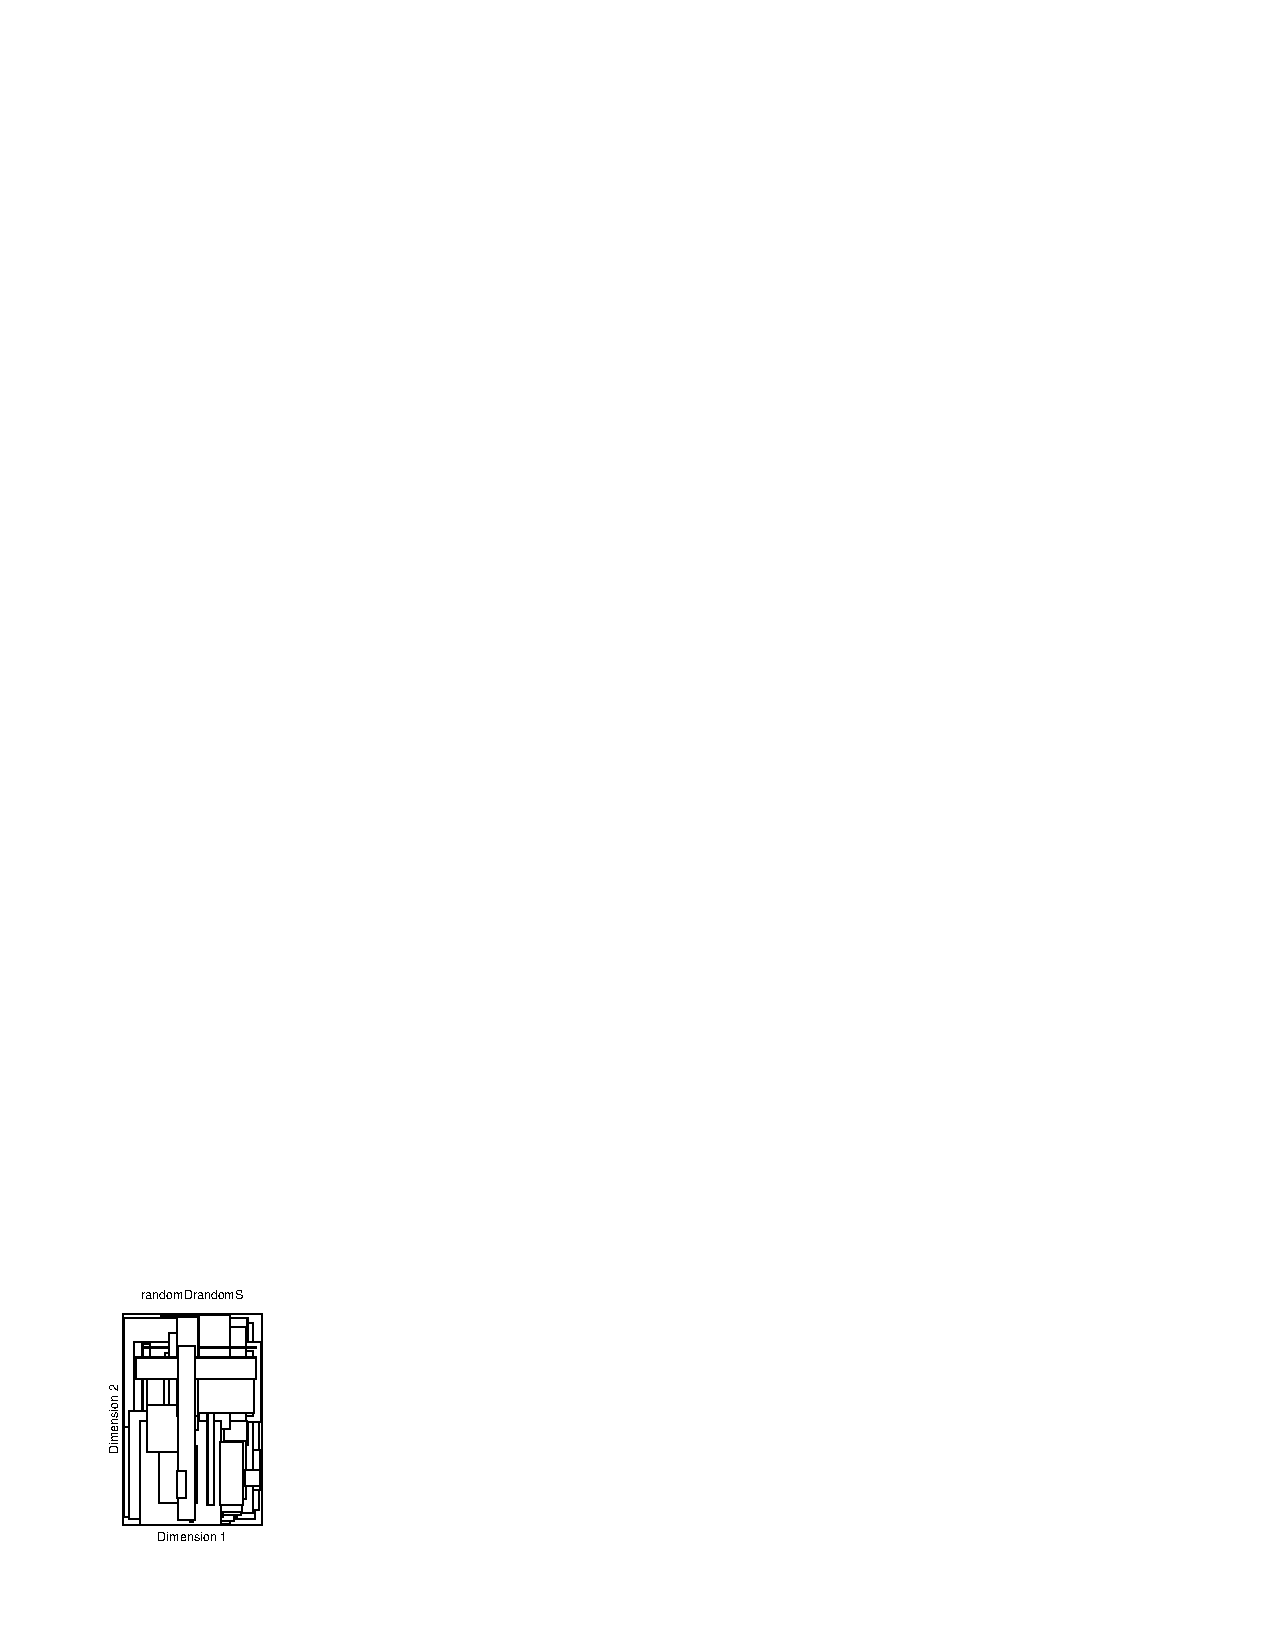
\includegraphics[trim=2.4cm 2.1cm 17cm 22cm]{Figures/queries/queries_randomDrandomS}
        }%
	\subfigure[]{%
            \label{fig:randomDsameS}
            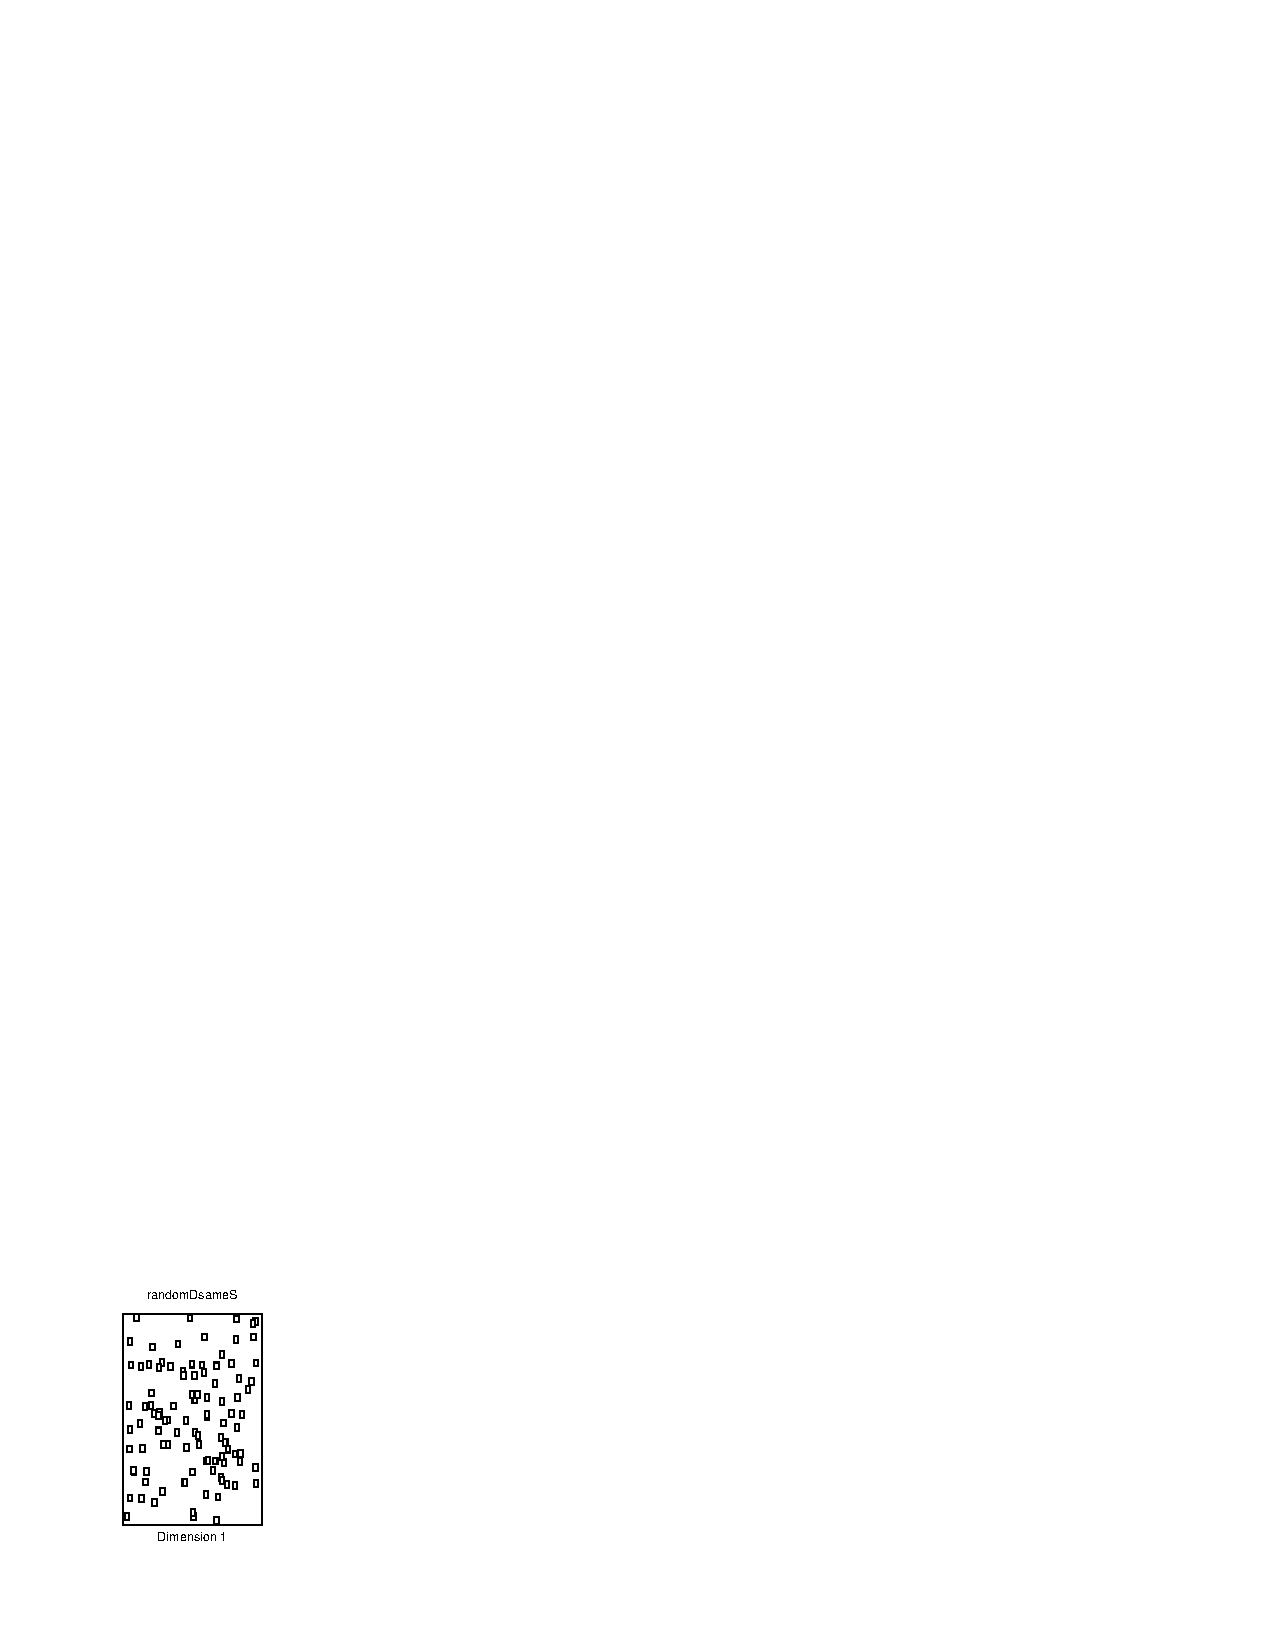
\includegraphics[trim=2.4cm 2.1cm 17cm 22cm]{Figures/queries/queries_randomDsameS}
        }%
        \subfigure[]{%
            \label{fig:randomDSBsameS}
            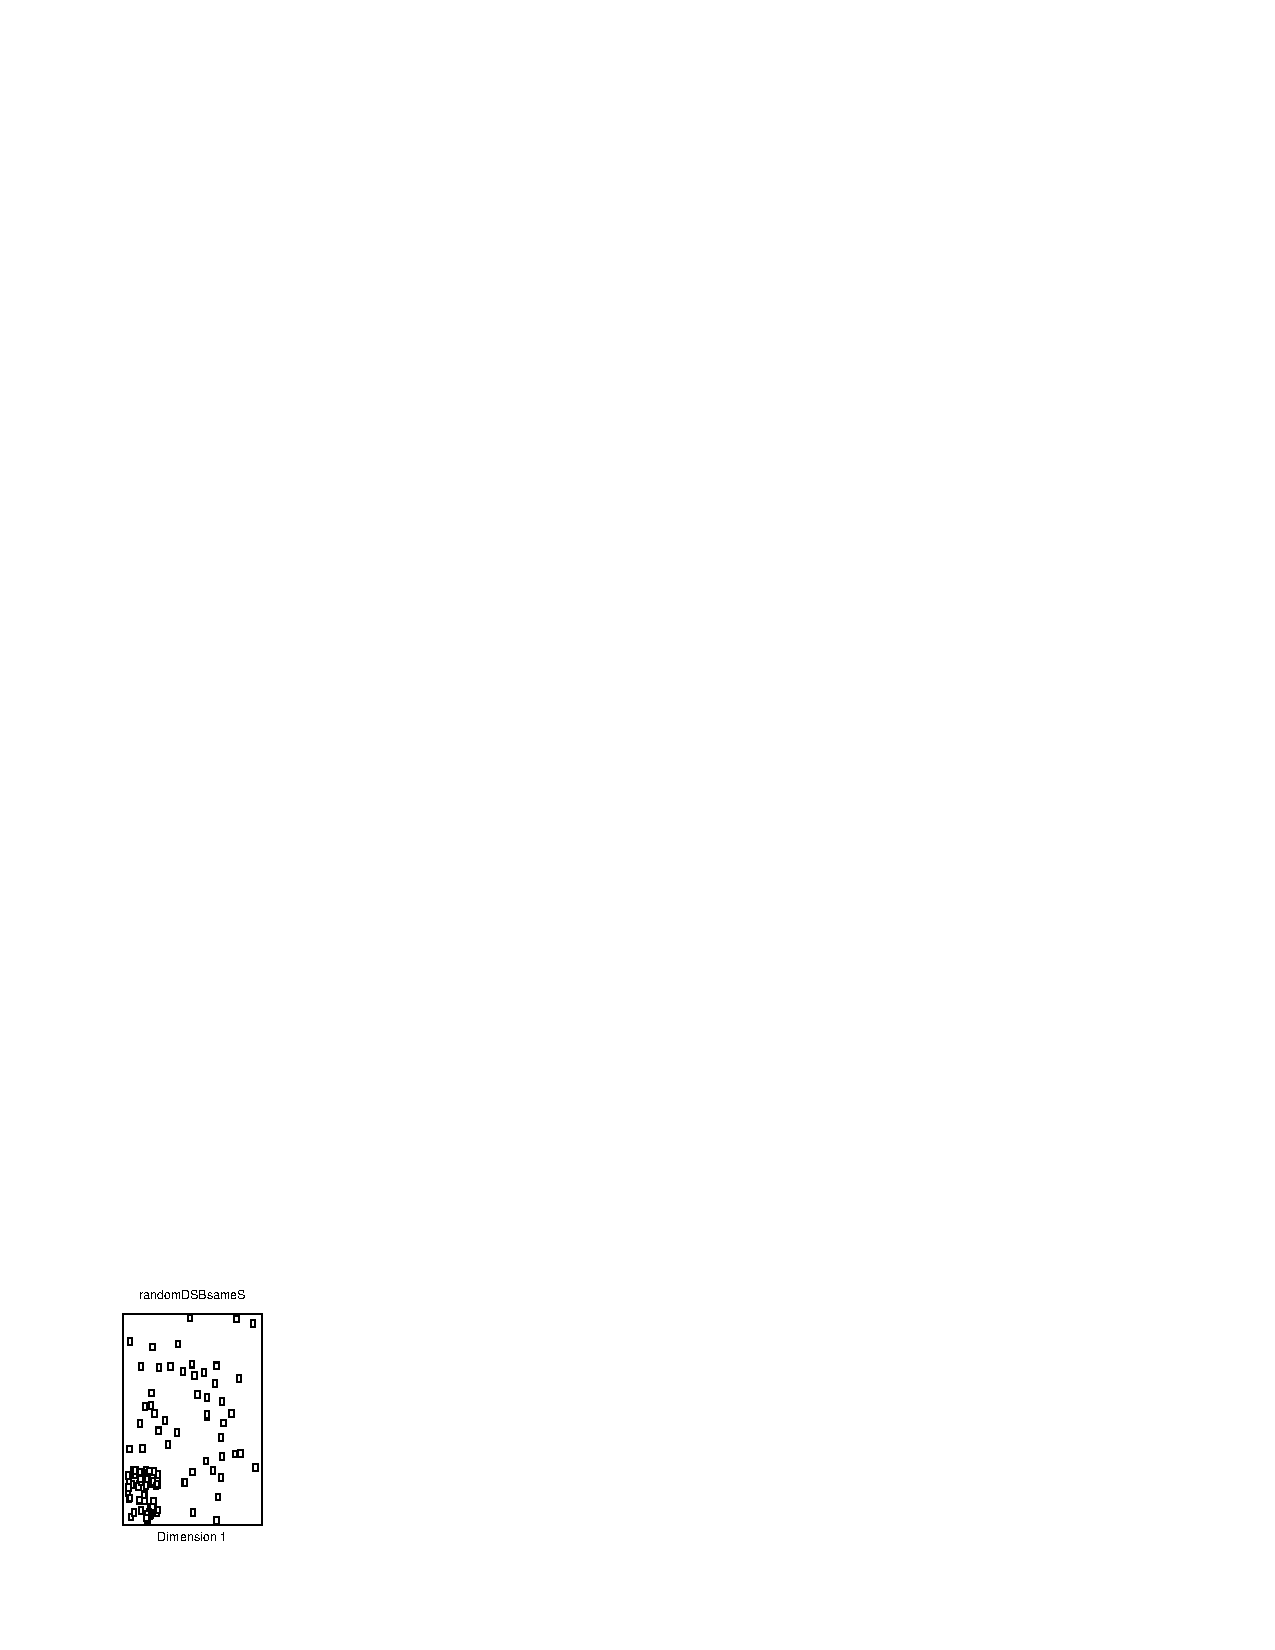
\includegraphics[trim=2.4cm 2.1cm 17cm 22cm]{Figures/queries/queries_randomDSBsameS}
        }%
	\subfigure[]{%
            \label{fig:skewedDsameS}
            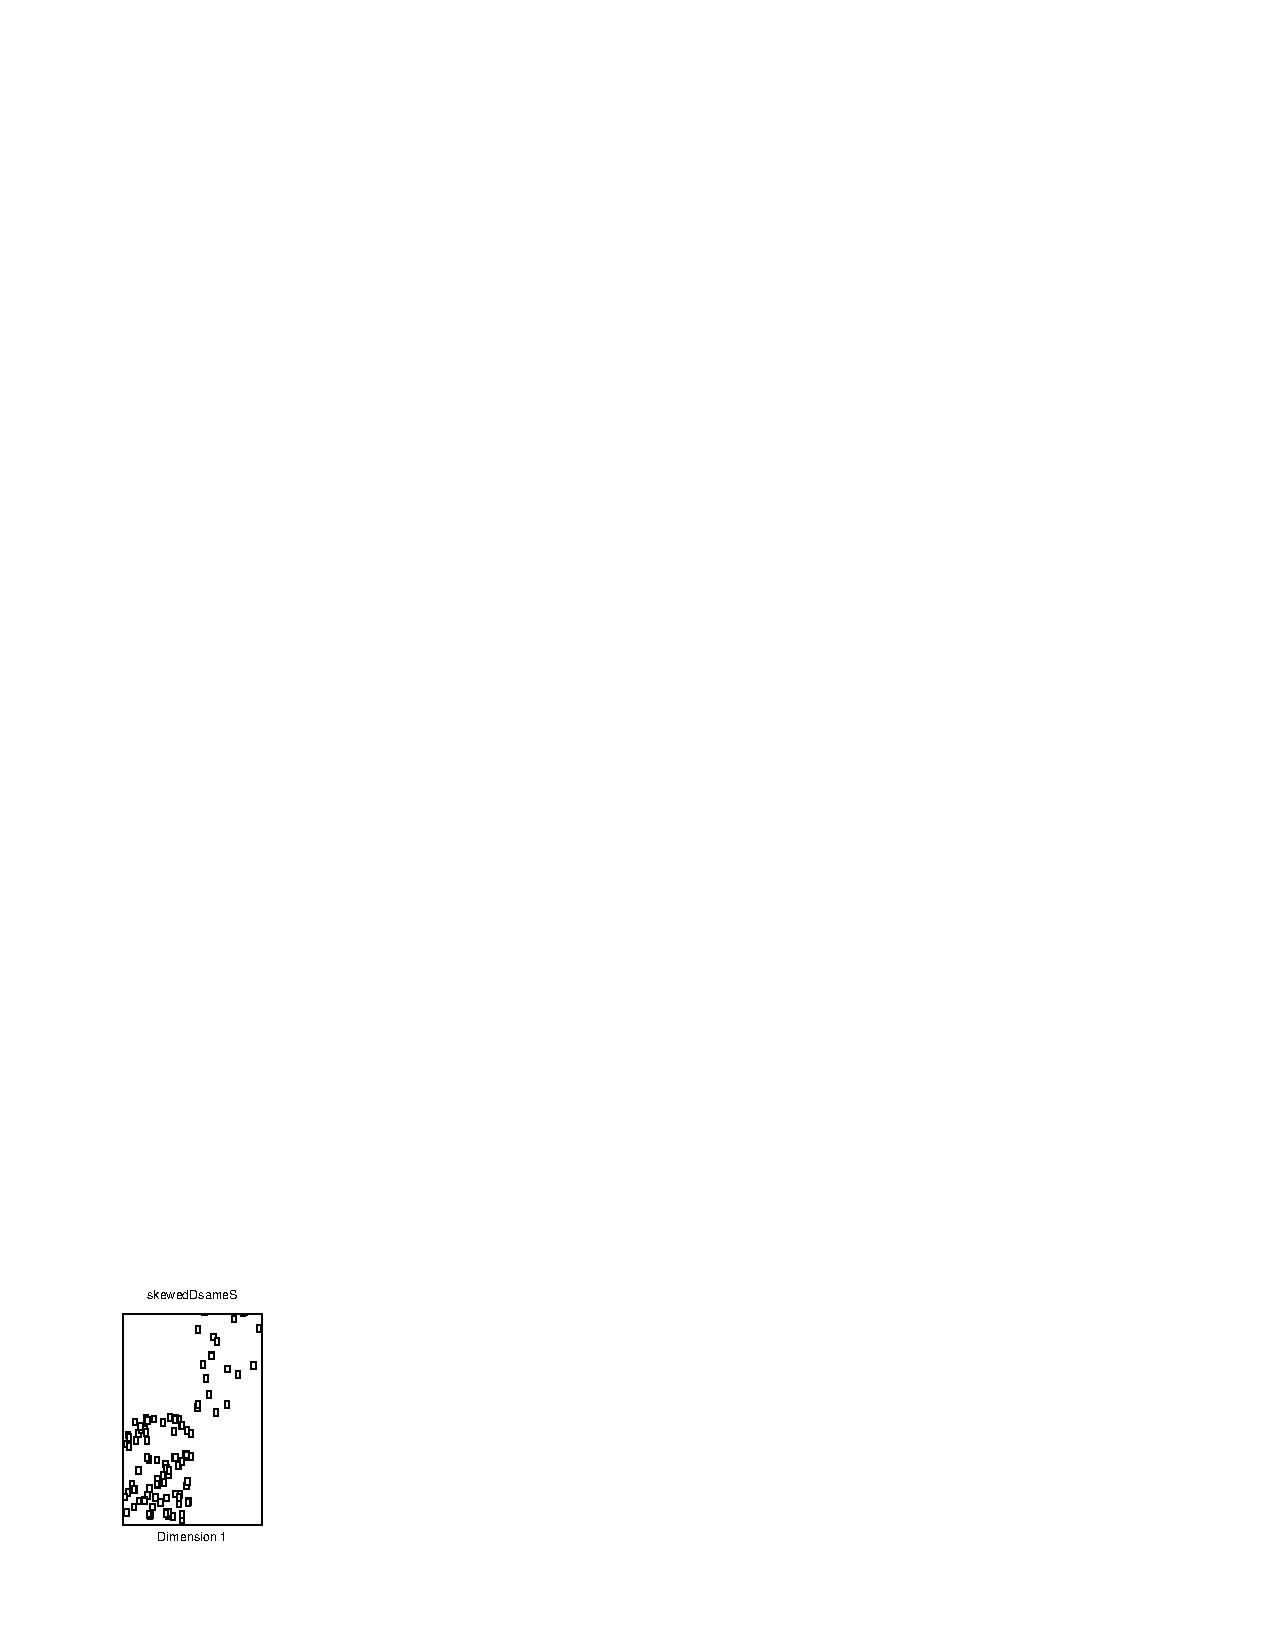
\includegraphics[trim=2.4cm 2.1cm 17cm 22cm]{Figures/queries/queries_skewedDsameS}
        }%
        \subfigure[]{%
            \label{fig:sequentialDsameS}
            
\includegraphics[trim=2.4cm 2.1cm 17cm 22cm]{Figures/queries/queries_sequentialDsameS}
        }%
	\subfigure[]{%
            \label{fig:periodicalDsameS}
            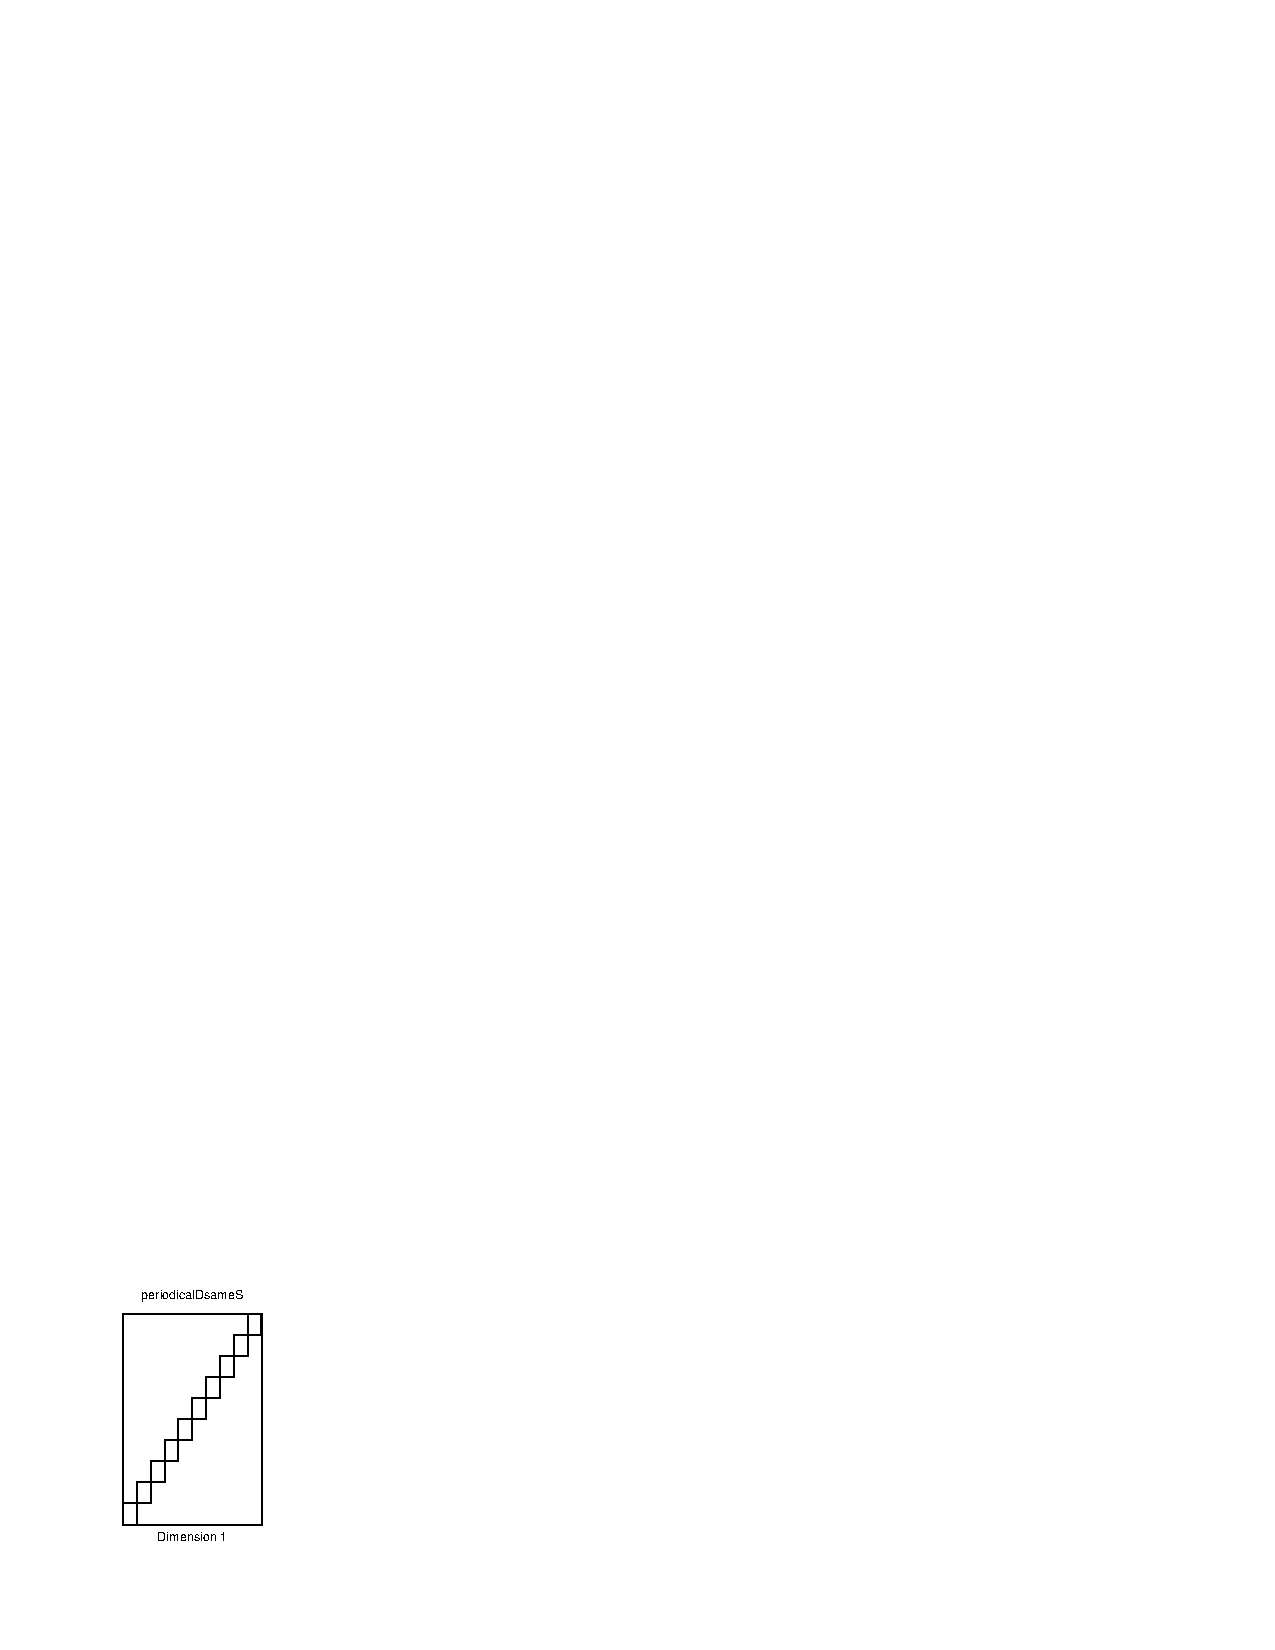
\includegraphics[trim=2.4cm 2.1cm 17cm 22cm]{Figures/queries/queries_periodicalDsameS}
        }%
	\subfigure[]{%
            \label{fig:zoominDdifferentS}
            
\includegraphics[trim=2.4cm 2.1cm 17cm 22cm]{Figures/queries/queries_zoominDdifferentS}
        }
    \caption{Projection of 100 2-dimensional range queries on a 2D plane.}
   \label{fig:workload}
    \end{center}
\end{figure*}

\begin{figure*}[t]
     \begin{center}
        \subfigure[]{%
            \label{fig:randomDrandomS_vs}
            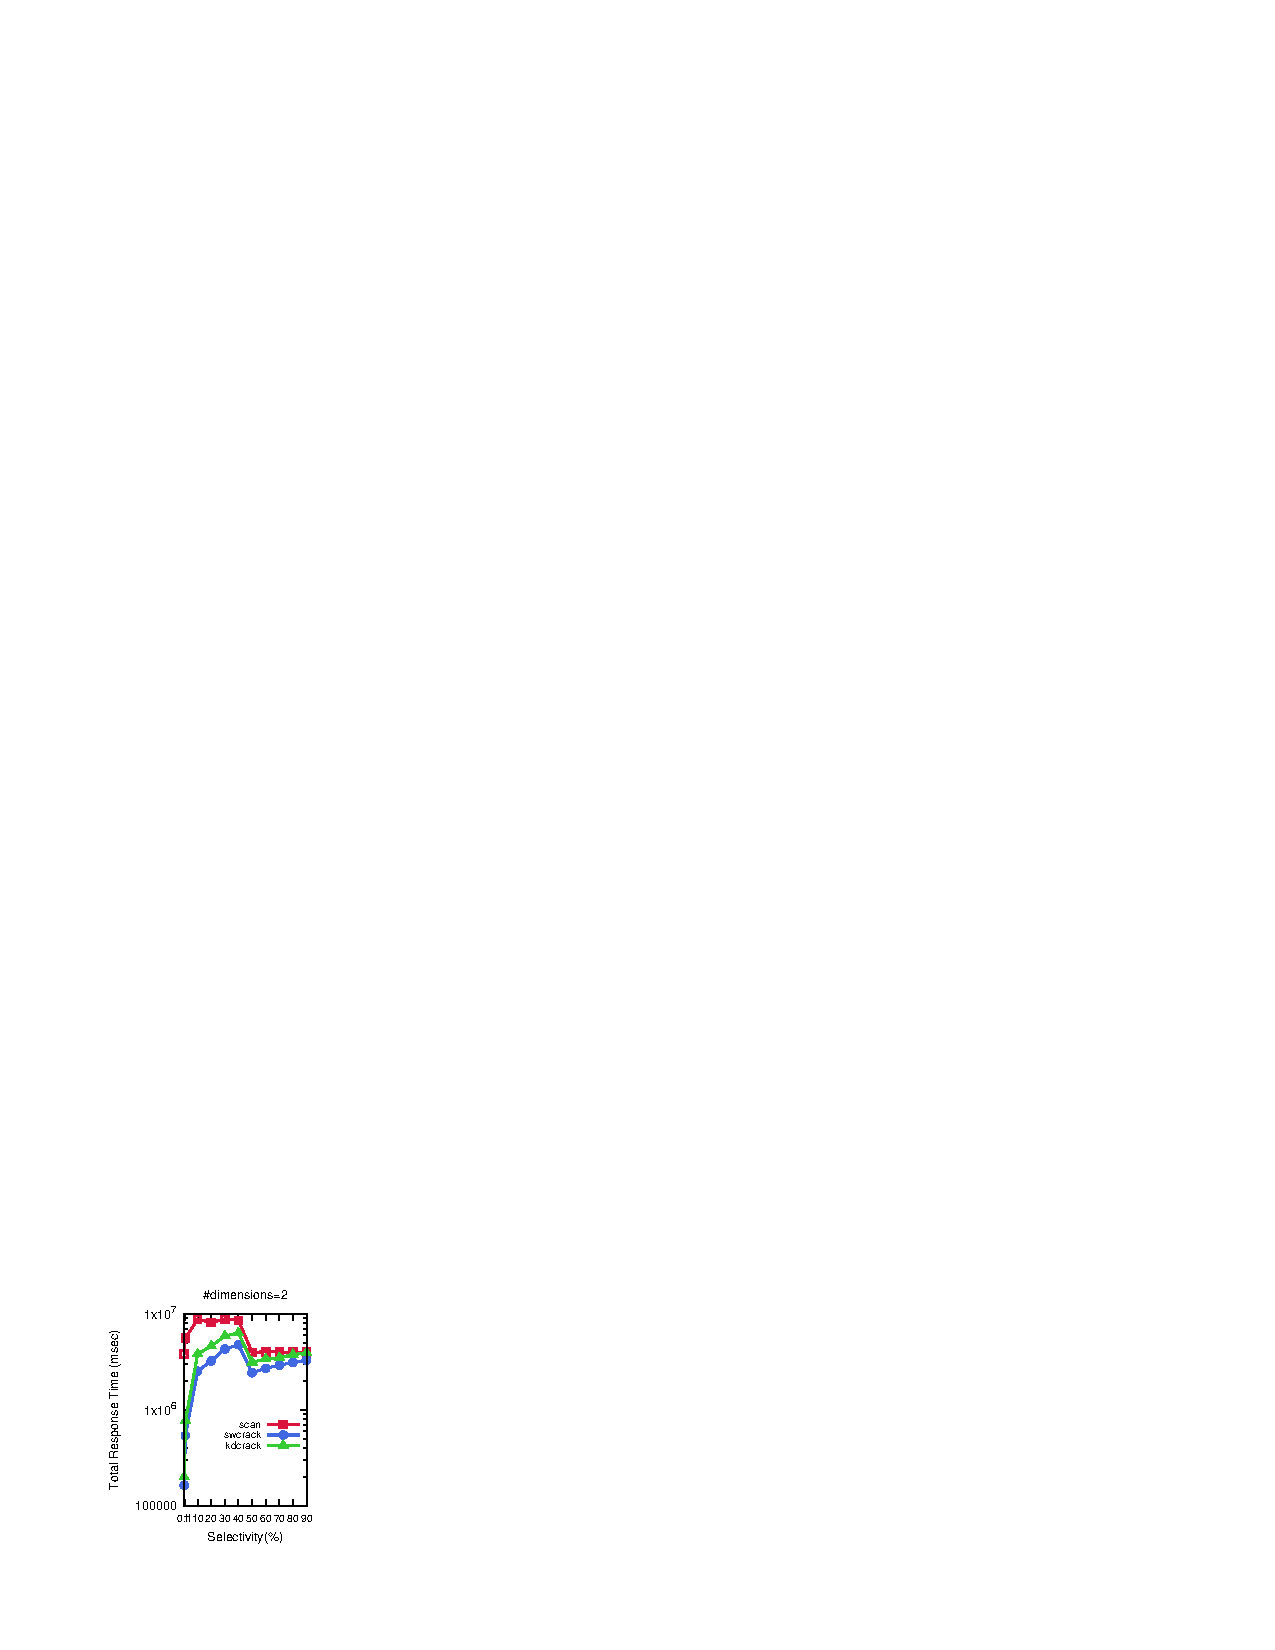
\includegraphics[trim=2cm 2.1cm 16.5cm 22cm]{Figures/vary_selectivity/2_1000_1000000.pdf}
        }%
	\subfigure[]{%
            \label{fig:randomDsameS_vs}
            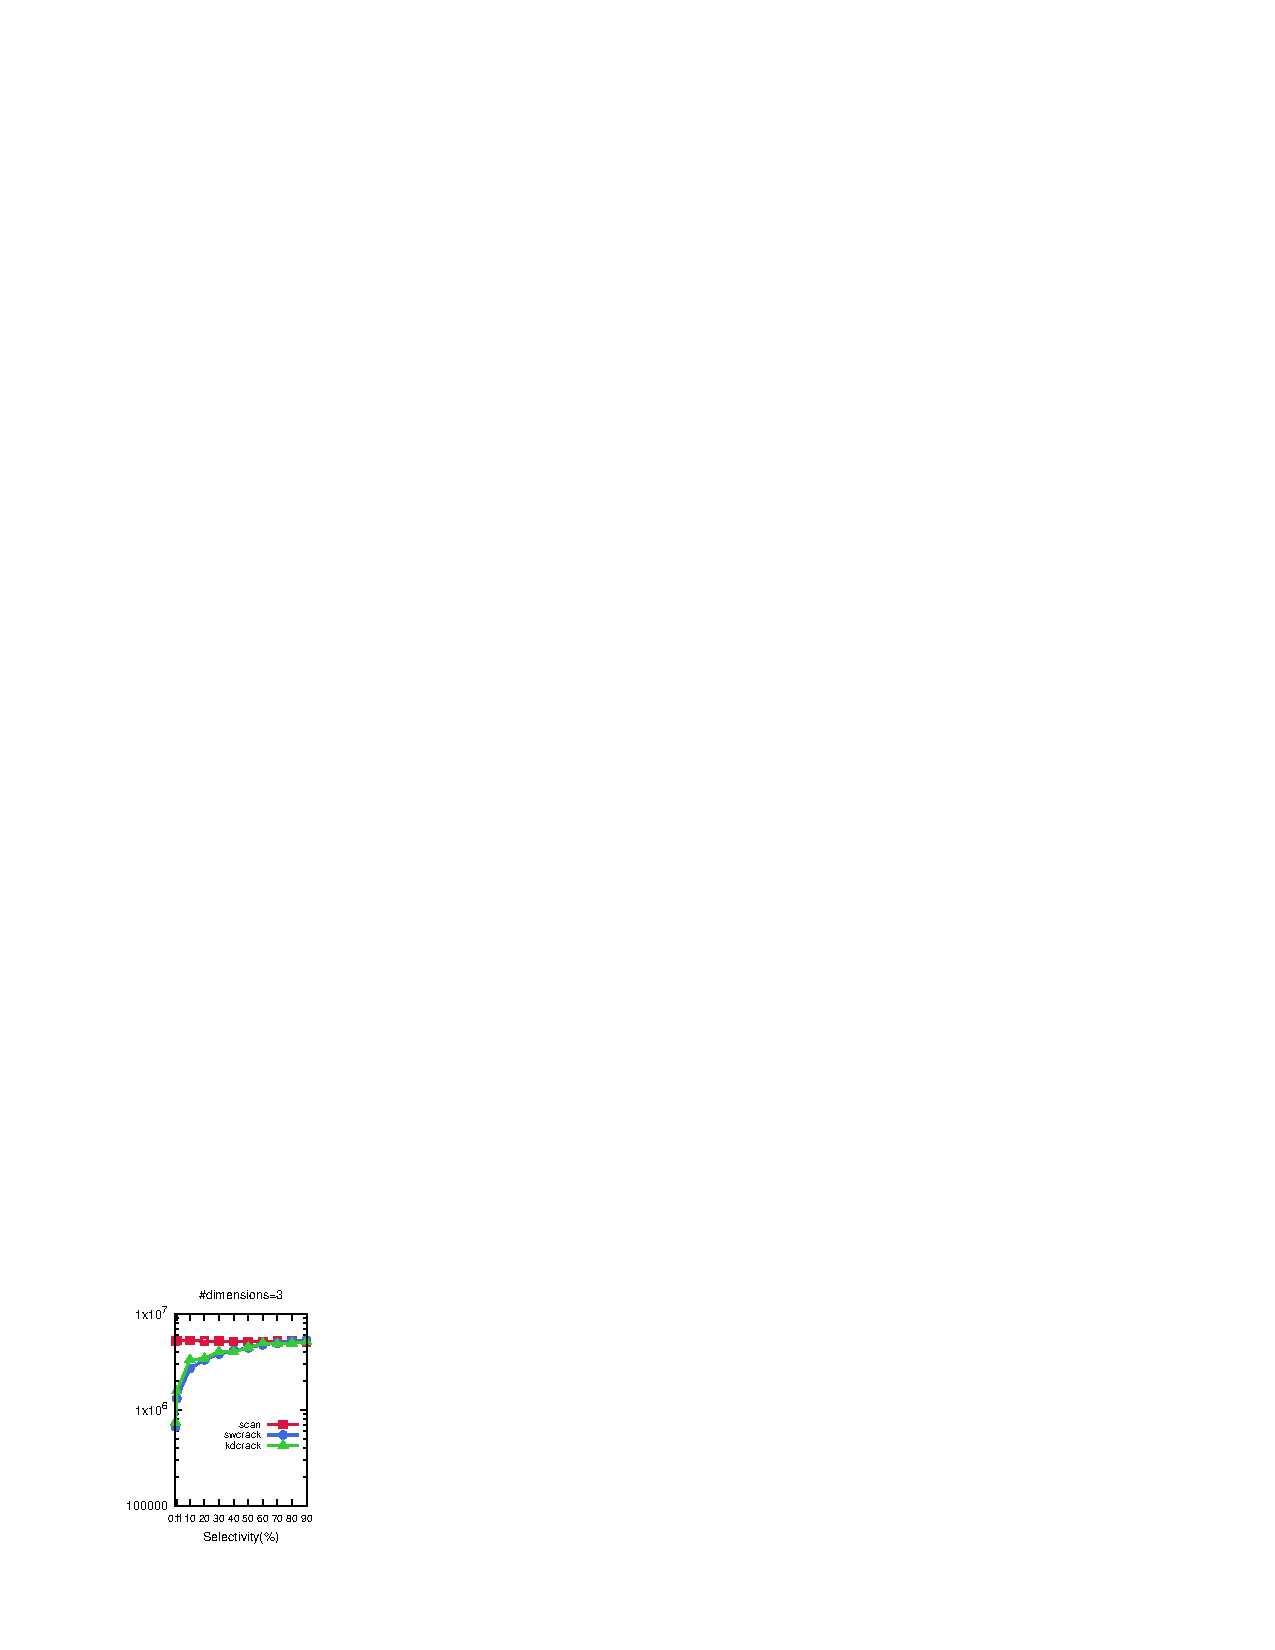
\includegraphics[trim=2cm 2.1cm 16.5cm 22cm]{Figures/vary_selectivity/3_1000_1000000.pdf}
        }%
        \subfigure[]{%
            \label{fig:randomDSBsameS_vs}
            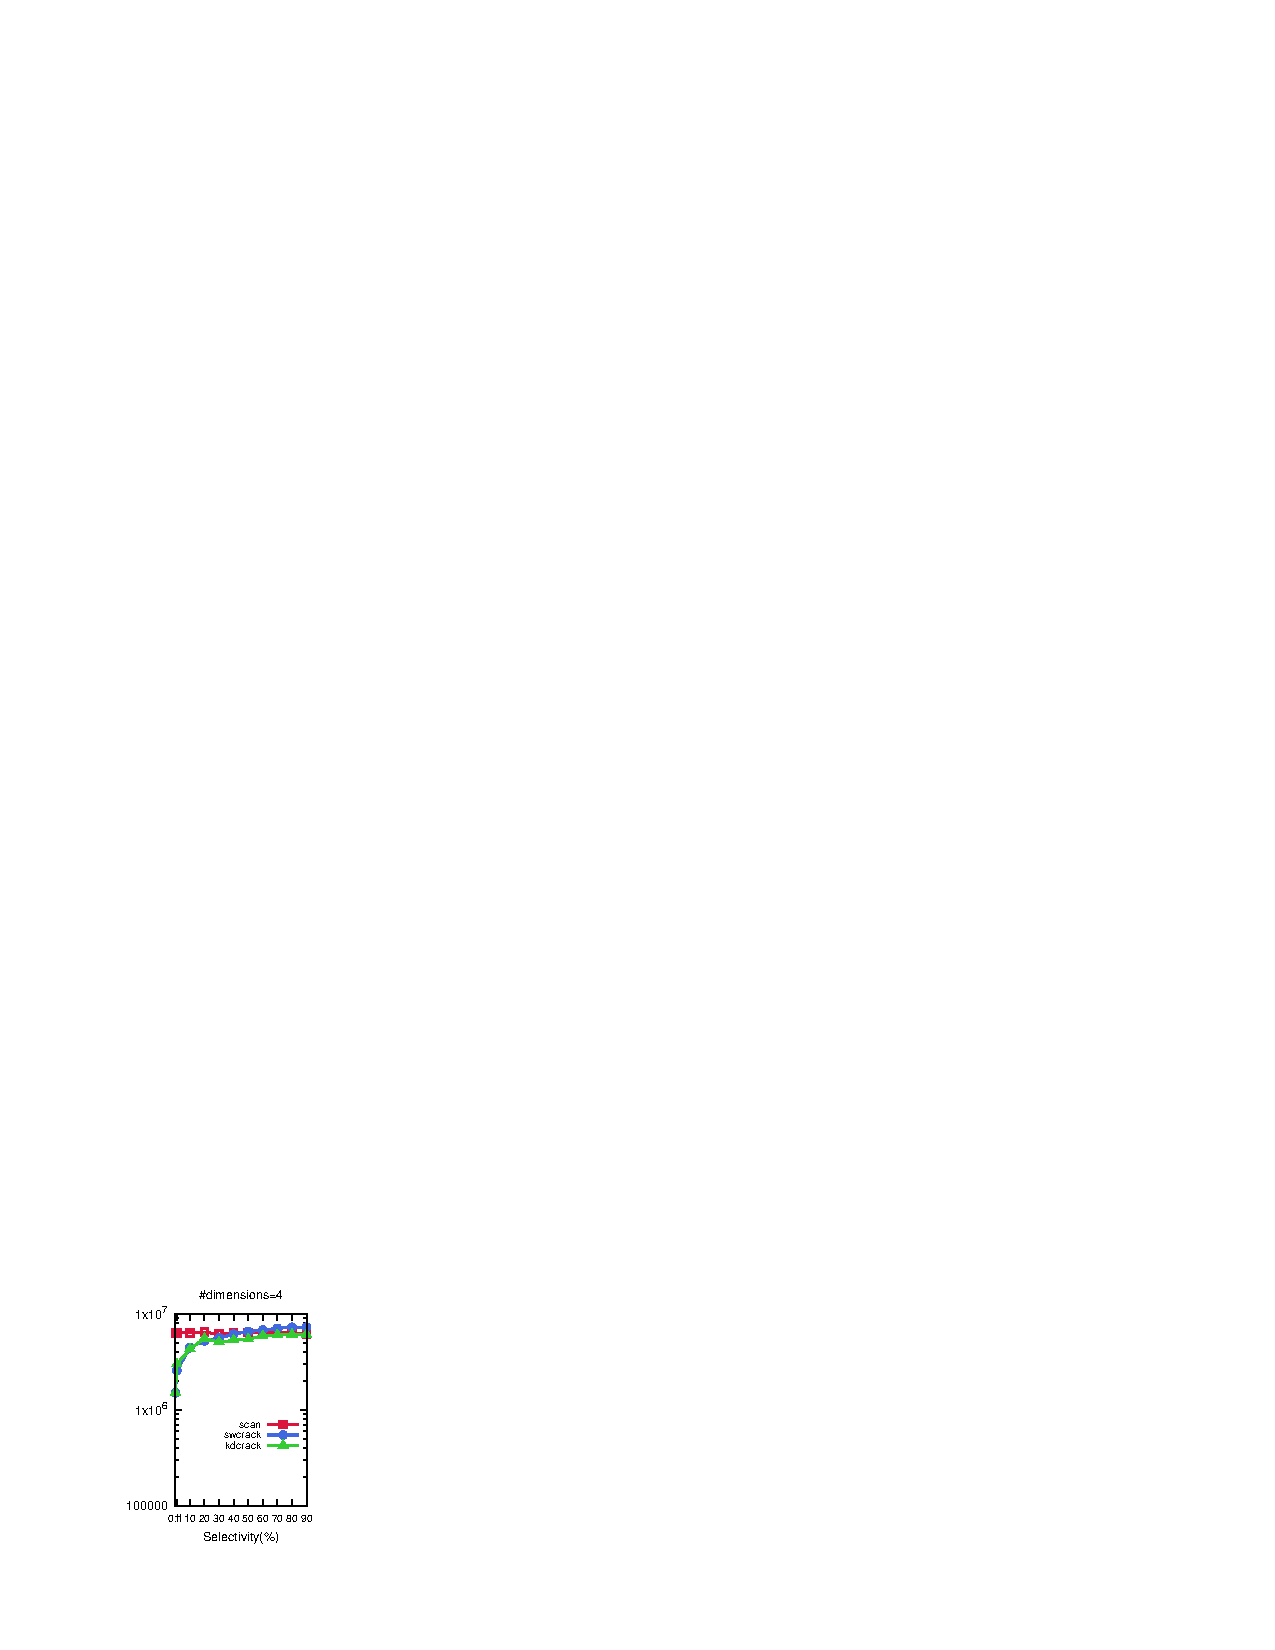
\includegraphics[trim=2cm 2.1cm 16.5cm 22cm]{Figures/vary_selectivity/4_1000_1000000.pdf}
        }%
	\subfigure[]{%
            \label{fig:skewedDsameS_vs}
            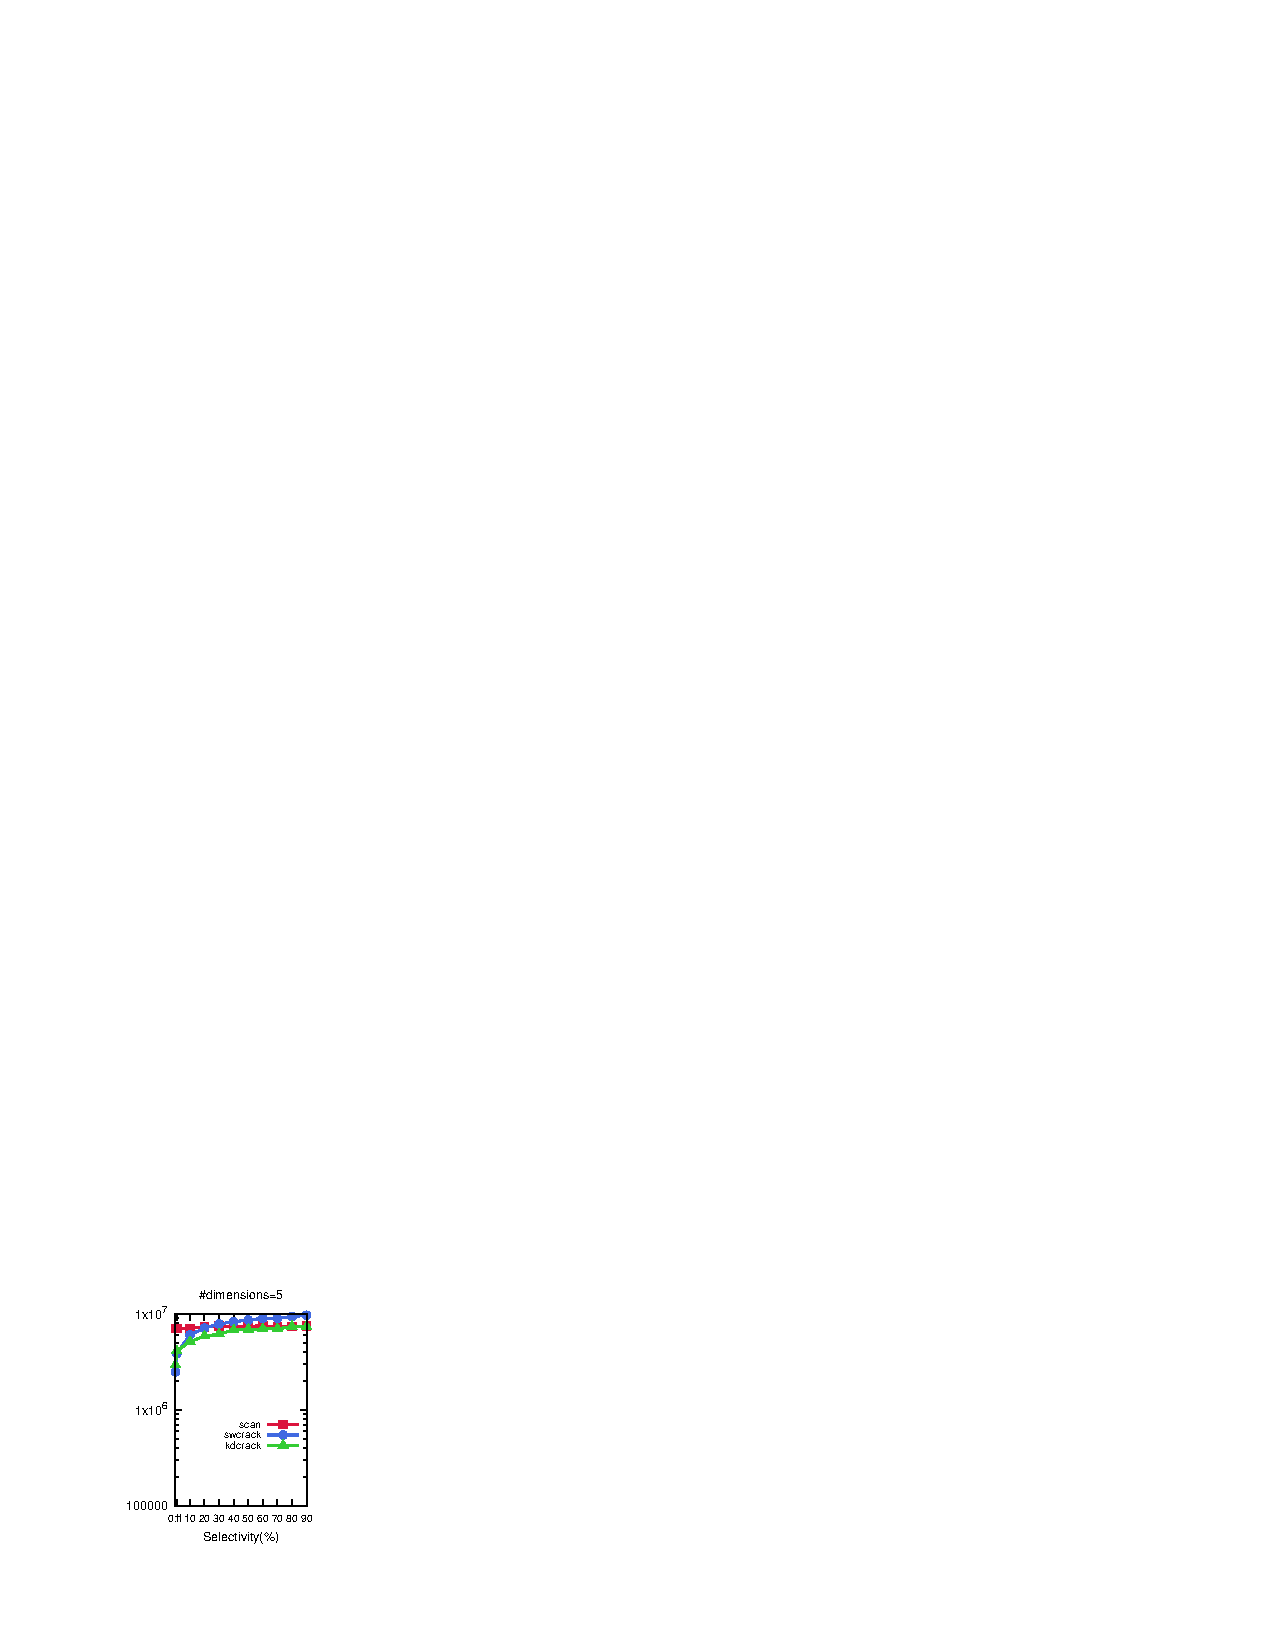
\includegraphics[trim=2cm 2.1cm 16.5cm 22cm]{Figures/vary_selectivity/5_1000_1000000.pdf}
        }%
        \subfigure[]{%
            \label{fig:sequentialDsameS_vs}
            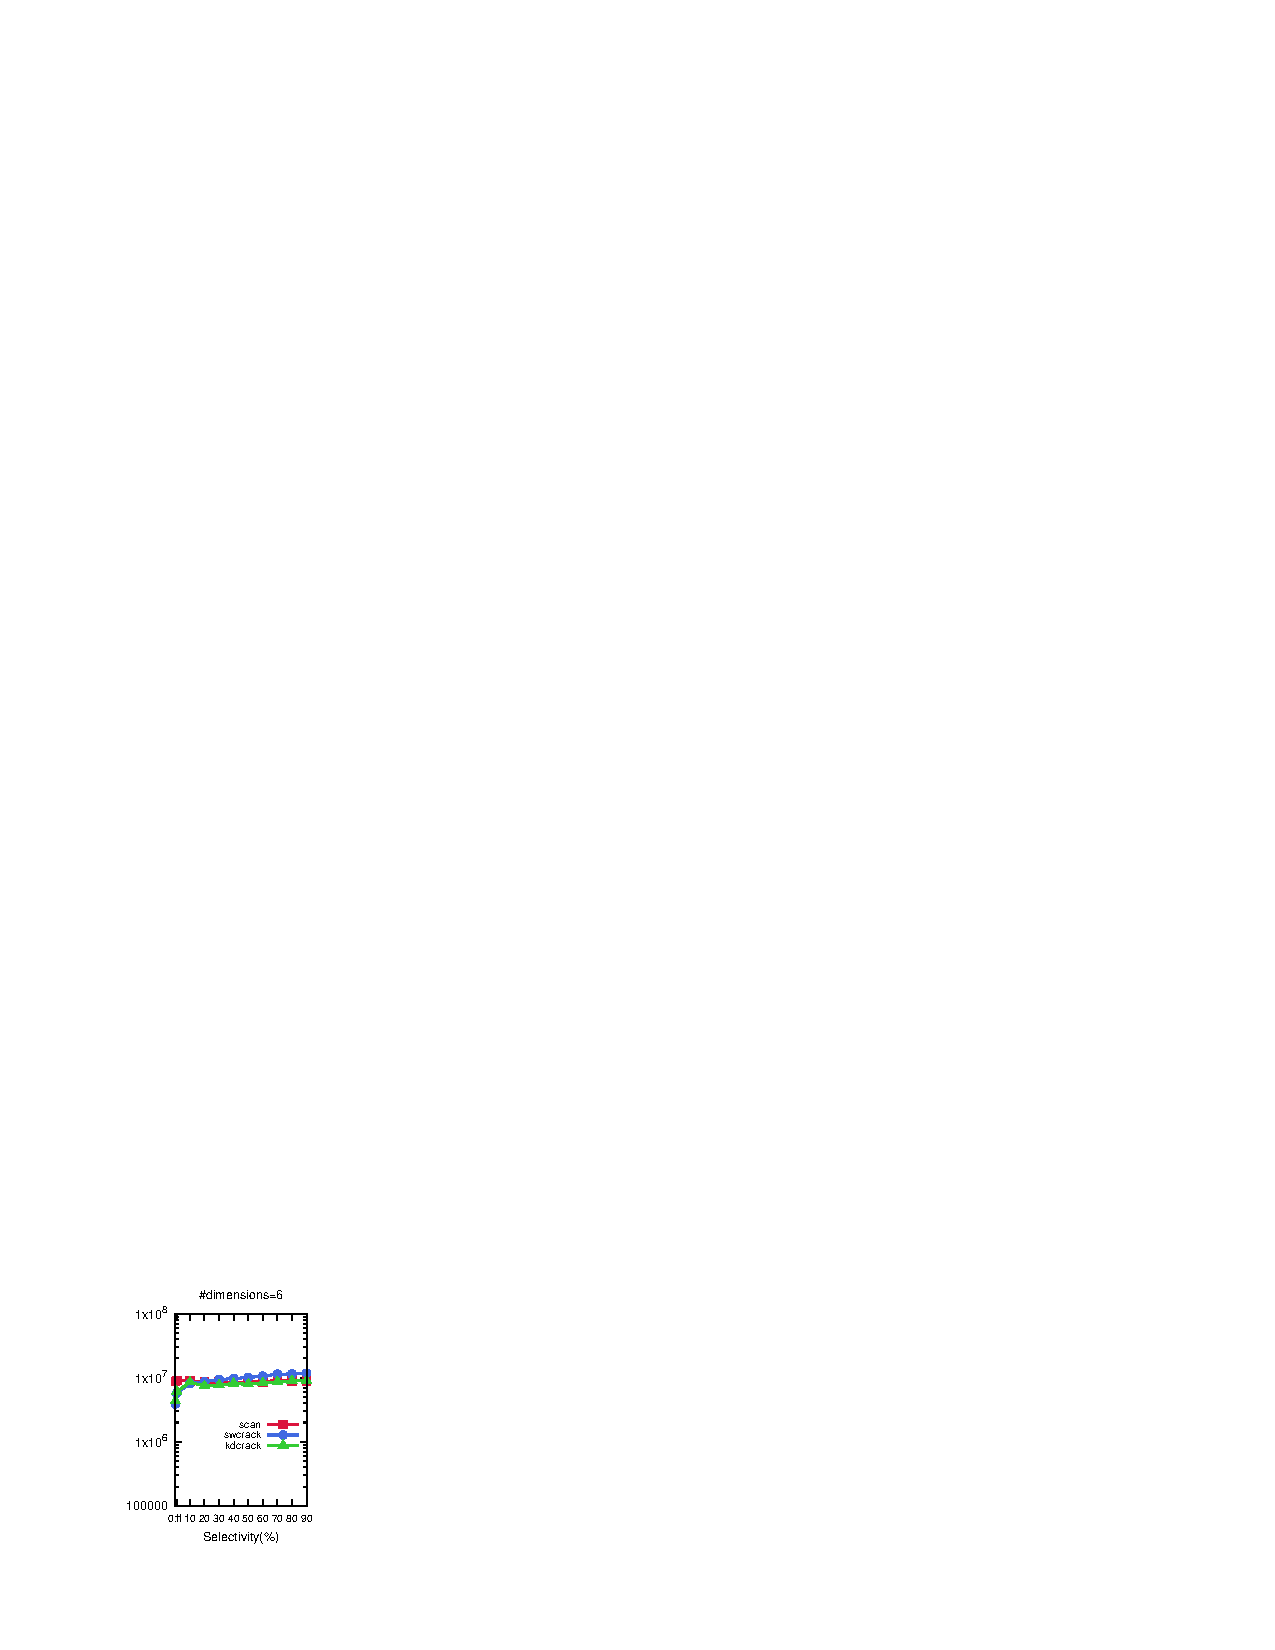
\includegraphics[trim=2cm 2.1cm 16.5cm 22cm]{Figures/vary_selectivity/6_1000_1000000.pdf}
        }    \caption{Varying selectivity of \emph{1000} queries for different $\#$dimensions (W=randomDsameS).}
   \label{fig:vary_selectivity}
    \end{center}
\end{figure*}

\begin{figure*}[t]
     \begin{center}
        \subfigure[]{%
            \label{fig:randomDrandomS}
            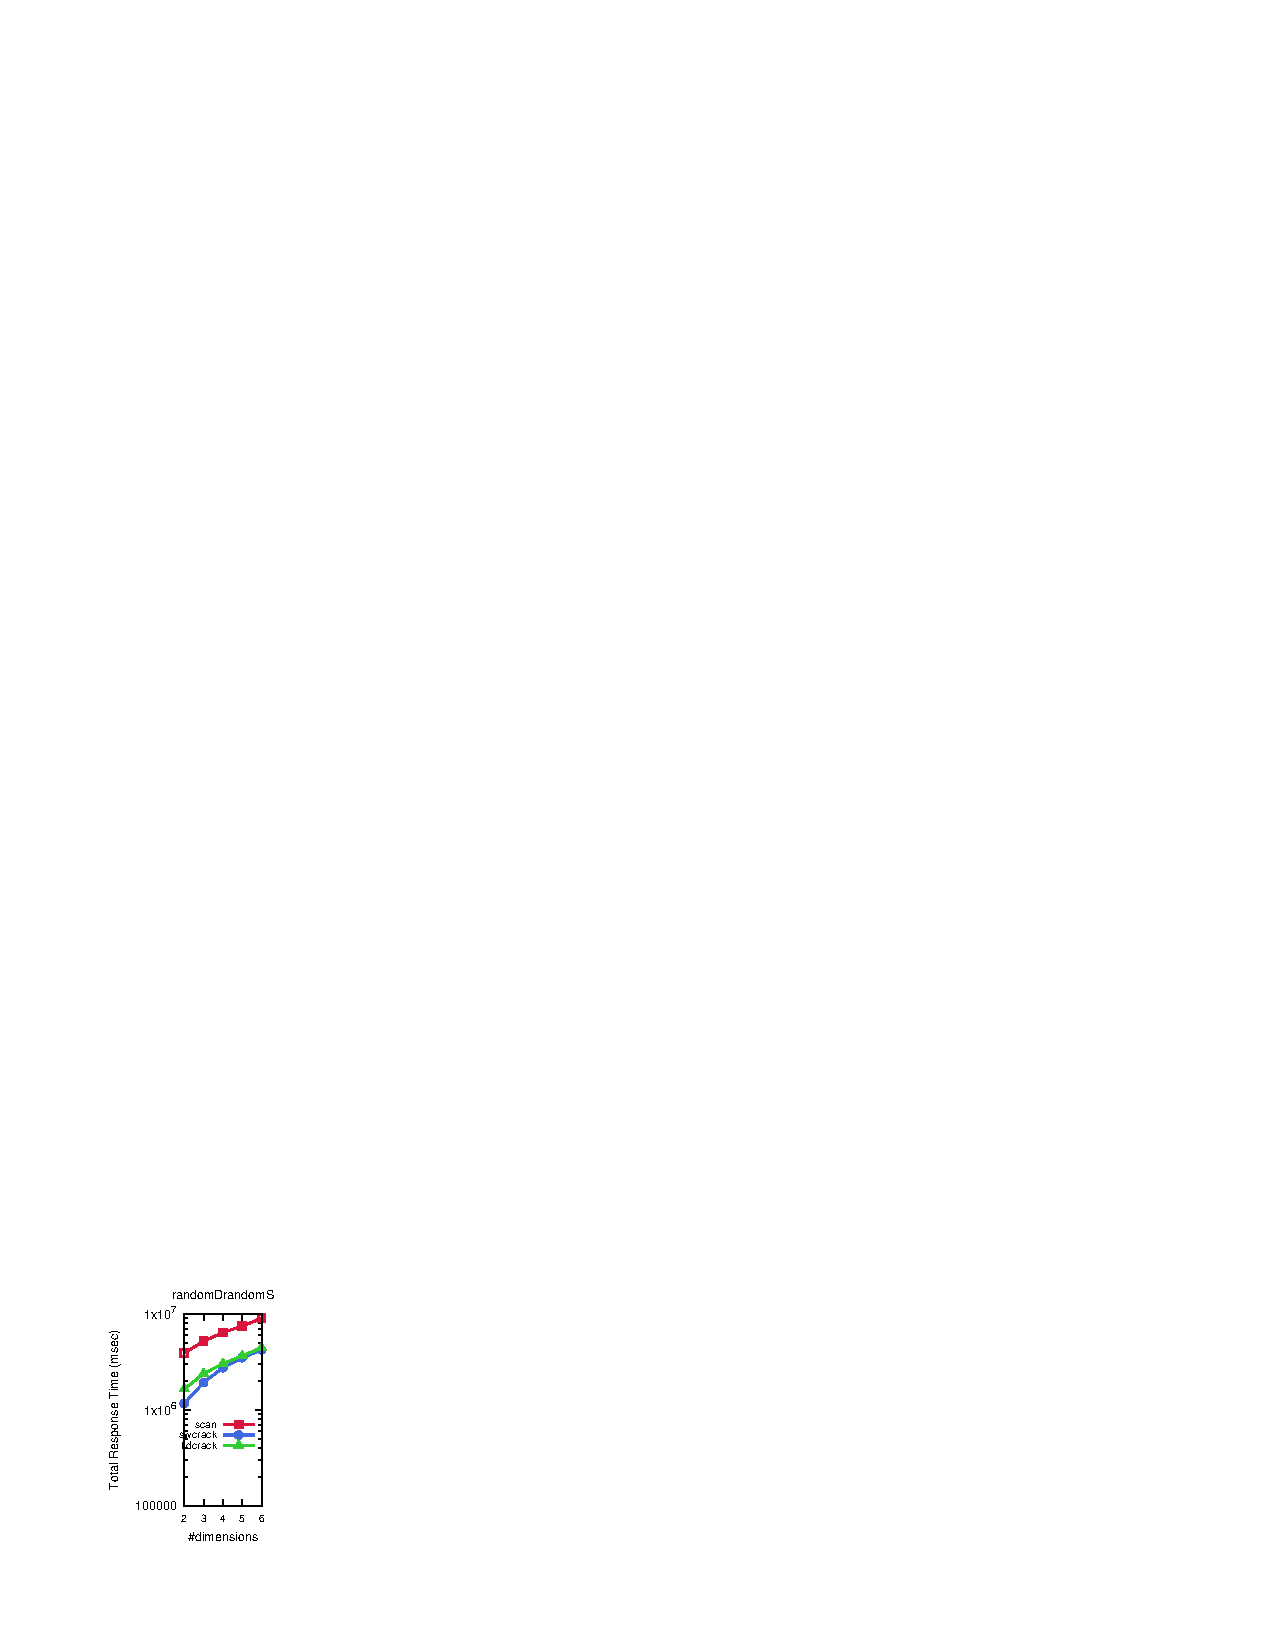
\includegraphics[trim=2.4cm 2.1cm 17cm 22cm]{Figures/vary_dimensions/randomDrandomS_vary_dimensions}
        }%
	\subfigure[]{%
            \label{fig:randomDsameS}
            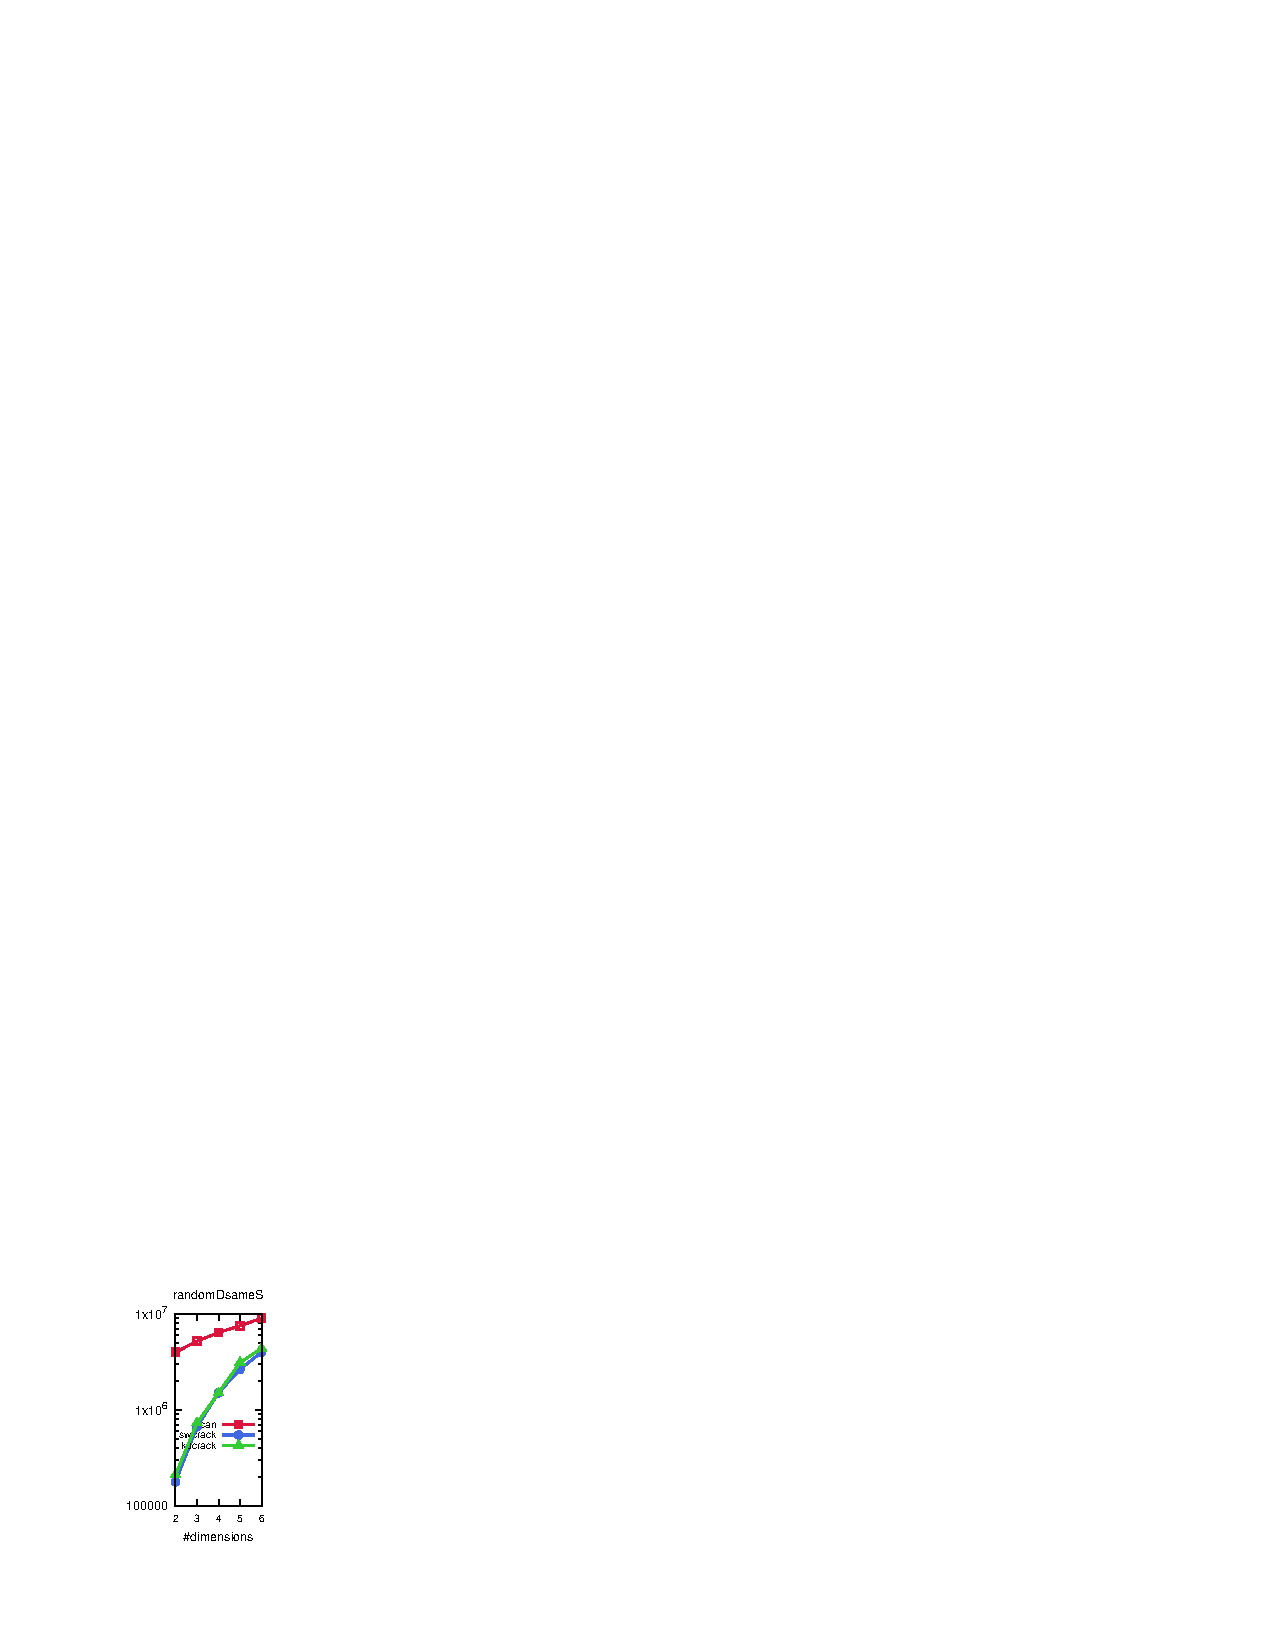
\includegraphics[trim=2.4cm 2.1cm 17cm 22cm]{Figures/vary_dimensions/randomDsameS_vary_dimensions}
        }%
        \subfigure[]{%
            \label{fig:randomDSBsameS}
            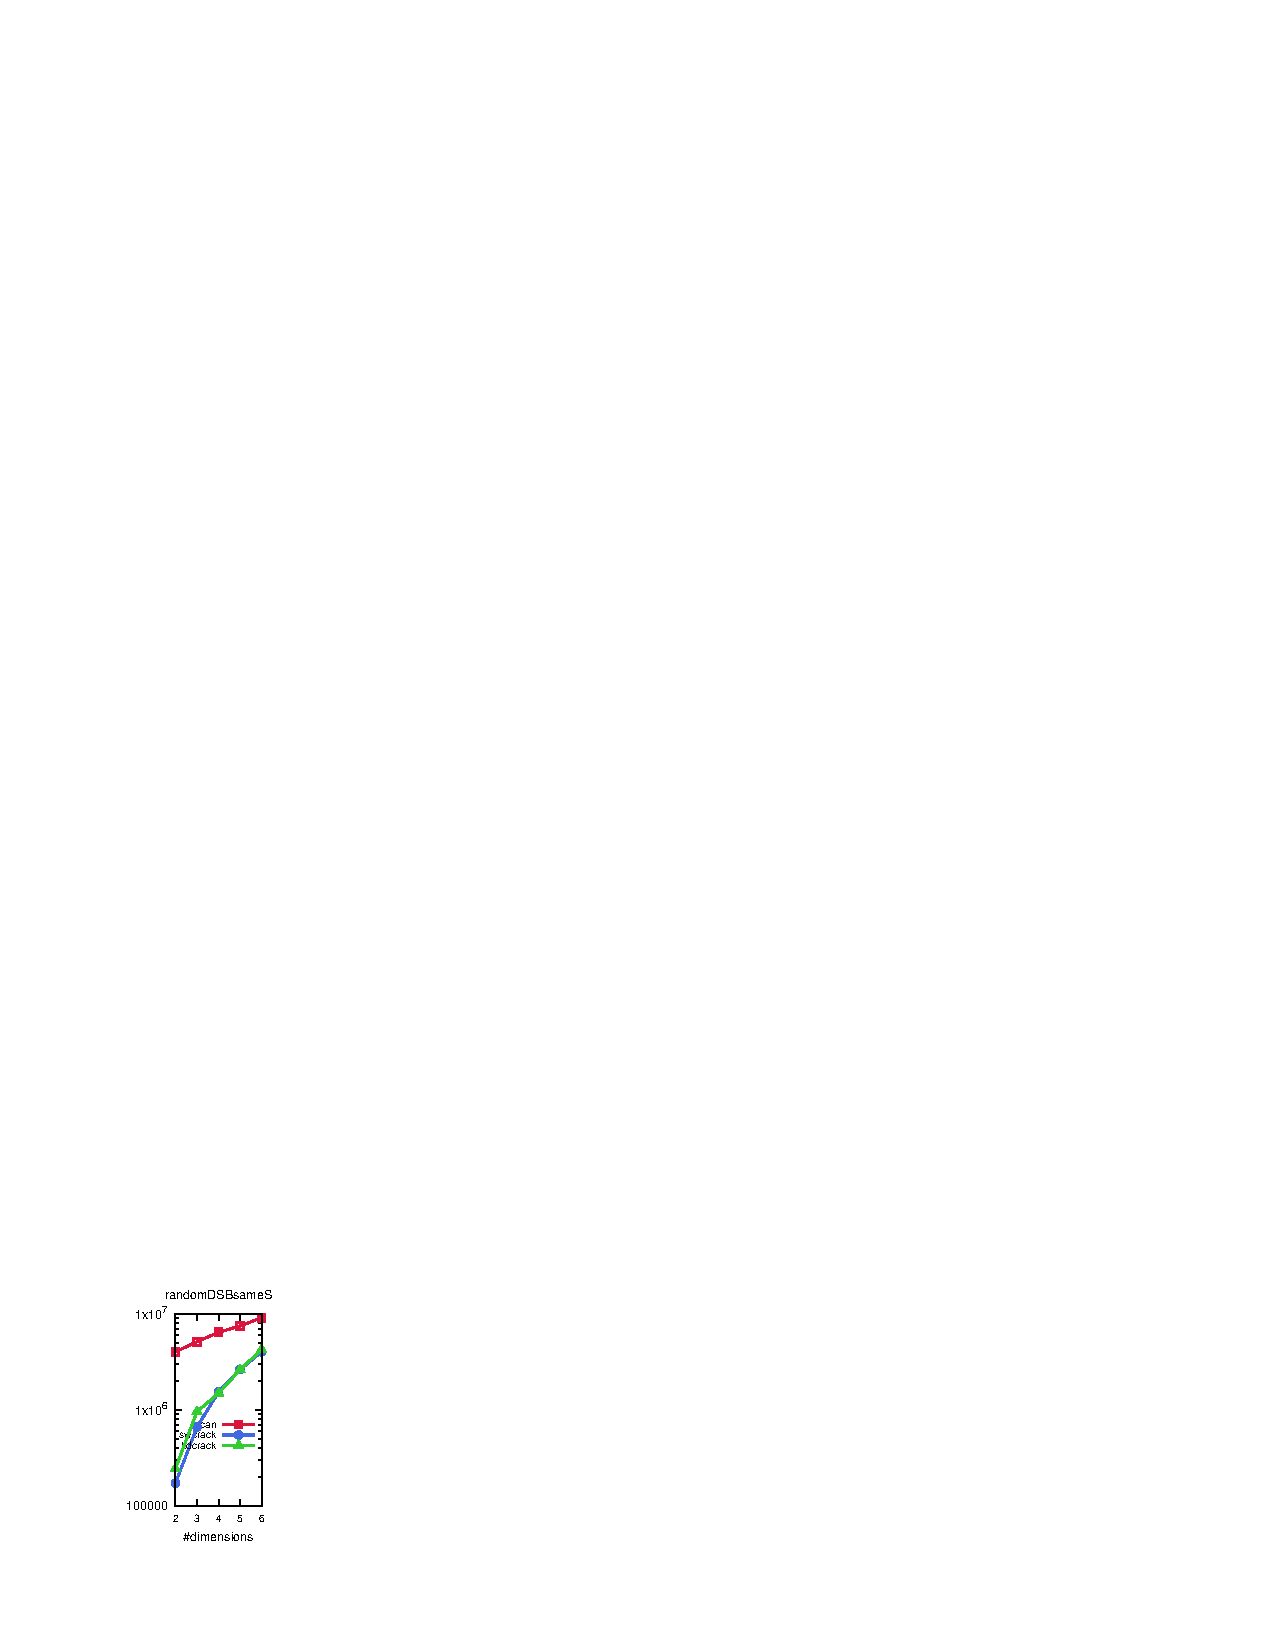
\includegraphics[trim=2.4cm 2.1cm 17cm 22cm]{Figures/vary_dimensions/randomDSBsameS_vary_dimensions}
        }%
	\subfigure[]{%
            \label{fig:skewedDsameS}
            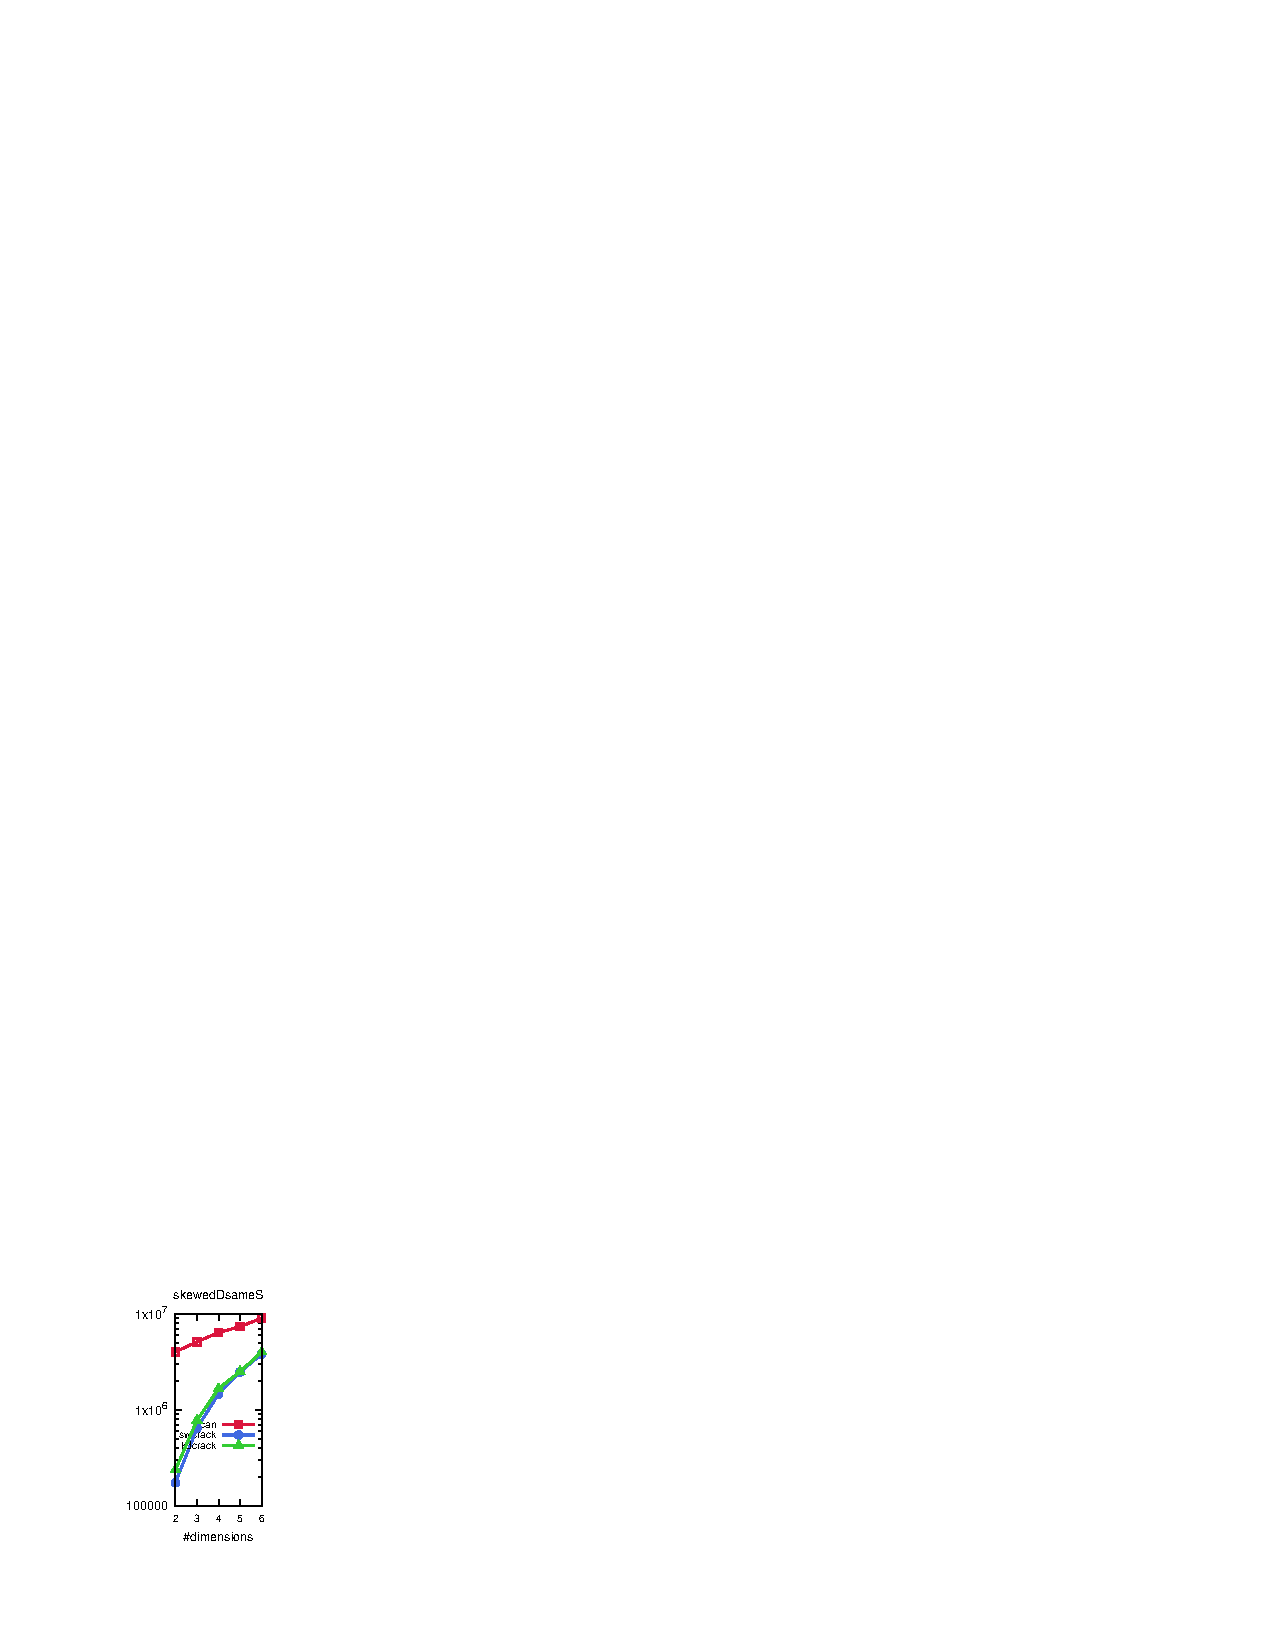
\includegraphics[trim=2.4cm 2.1cm 17cm 22cm]{Figures/vary_dimensions/skewedDsameS_vary_dimensions}
        }%
        \subfigure[]{%
            \label{fig:sequentialDsameS}
            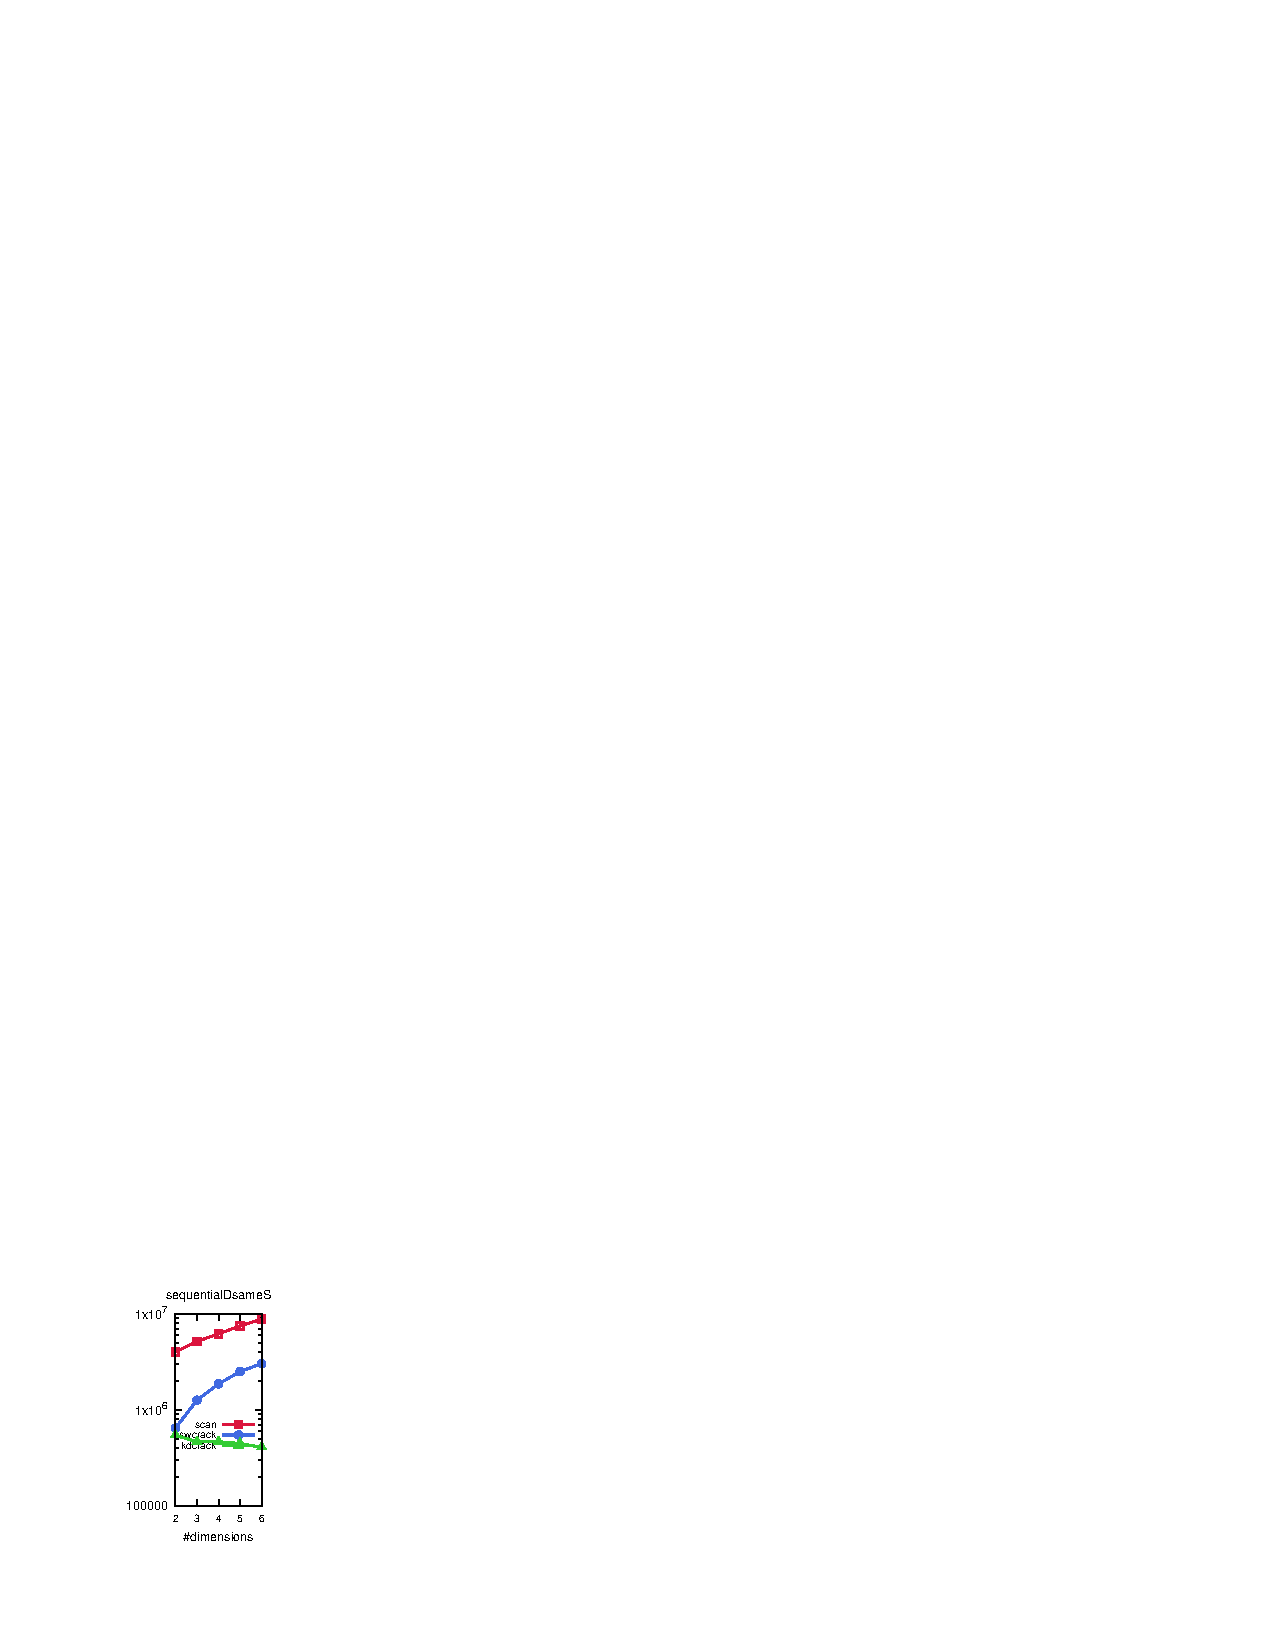
\includegraphics[trim=2.4cm 2.1cm 17cm 22cm]{Figures/vary_dimensions/sequentialDsameS_vary_dimensions}
        }%
	\subfigure[]{%
            \label{fig:periodicalDsameS}
            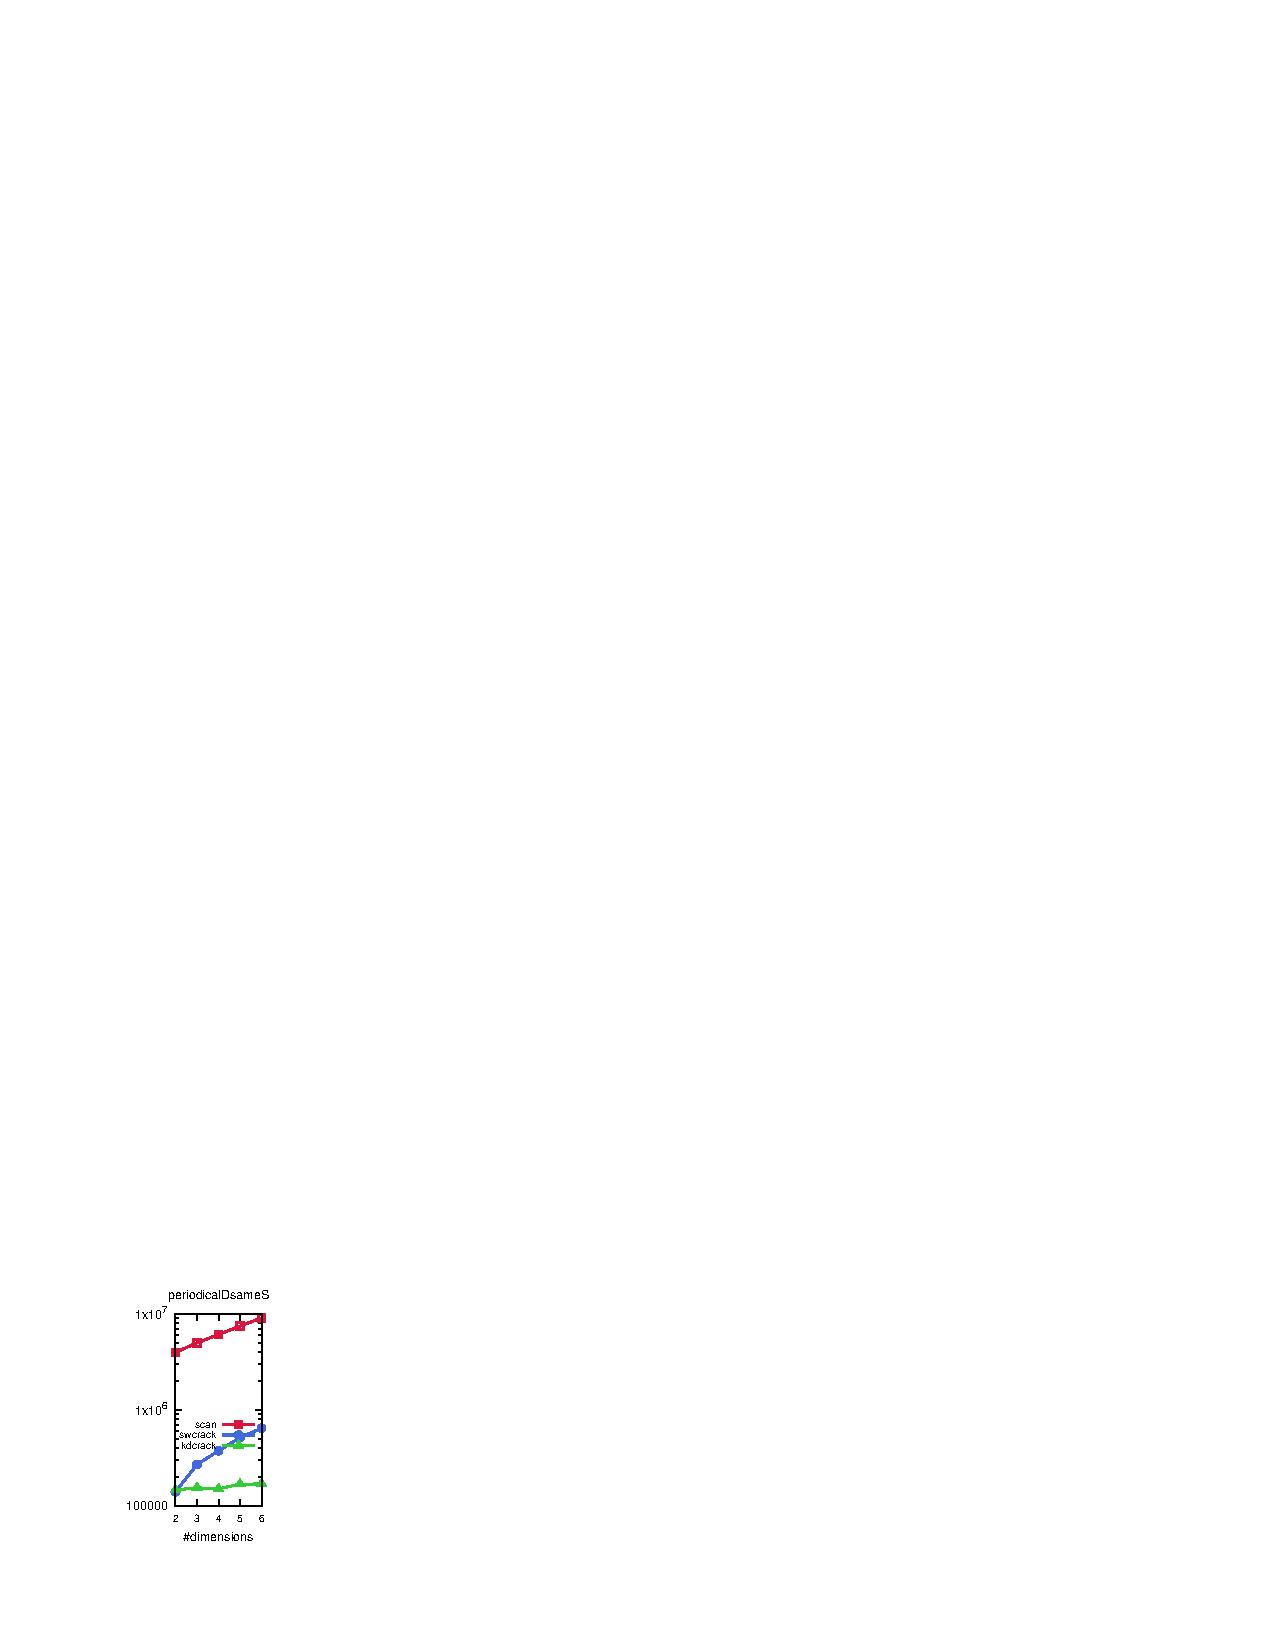
\includegraphics[trim=2.4cm 2.1cm 17cm 22cm]{Figures/vary_dimensions/periodicalDsameS_vary_dimensions}
        }%
	\subfigure[]{%
            \label{fig:zoominDdifferentS}
            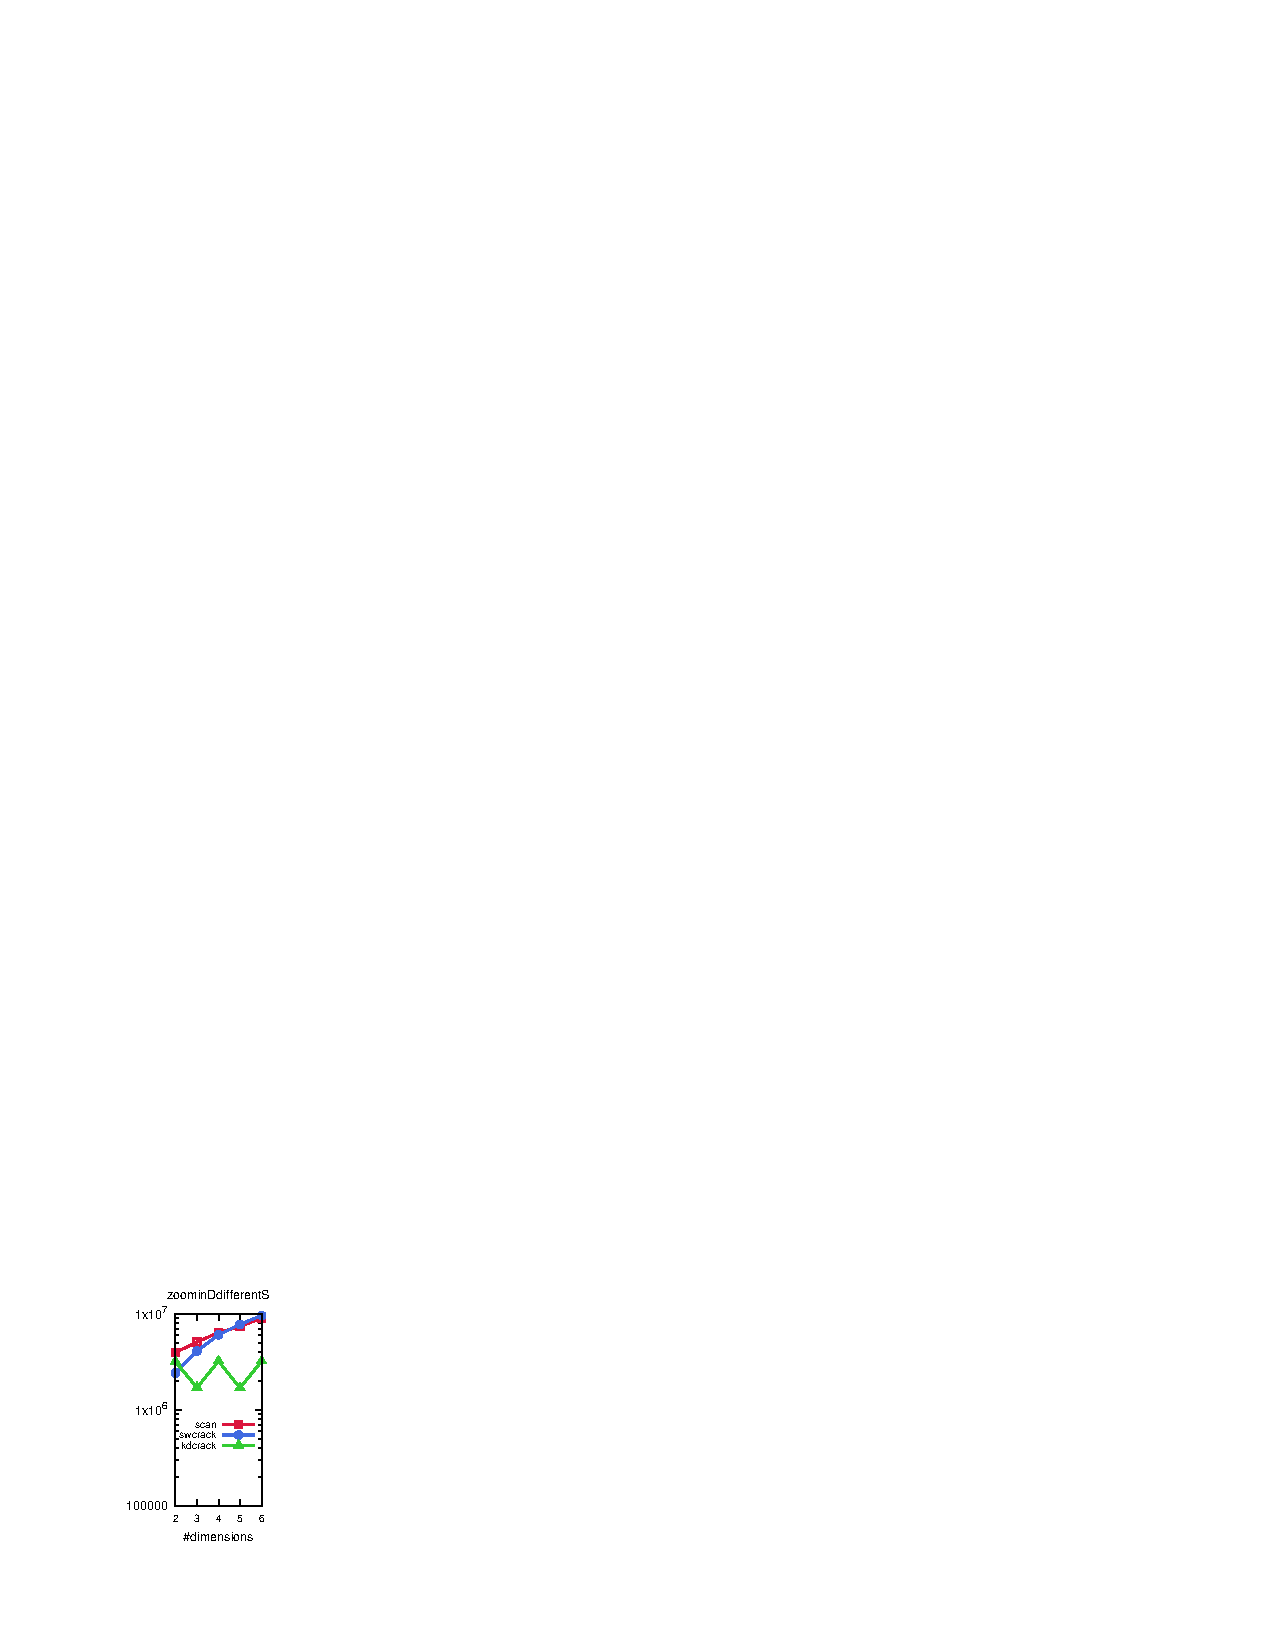
\includegraphics[trim=2.4cm 2.1cm 17cm 22cm]{Figures/vary_dimensions/zoominDdifferentS_vary_dimensions}
        }
    \caption{Varying $\#$dimensions of \emph{1000} queries for different workloads.}
   \label{fig:vary_dimensions}
    \end{center}
\end{figure*}


\textbf{Hardware/Software description.}

\textbf{Microbenchmark description.}

It would be nice if we included at least one experiment with real data or a standard benchmark like tpch.
Look if skyserver can be a useful example here.

\textbf{Experiments.}


\begin{figure*}[t]
     \begin{center}
        \subfigure[]{%
            \label{fig:randomDrandomS}
            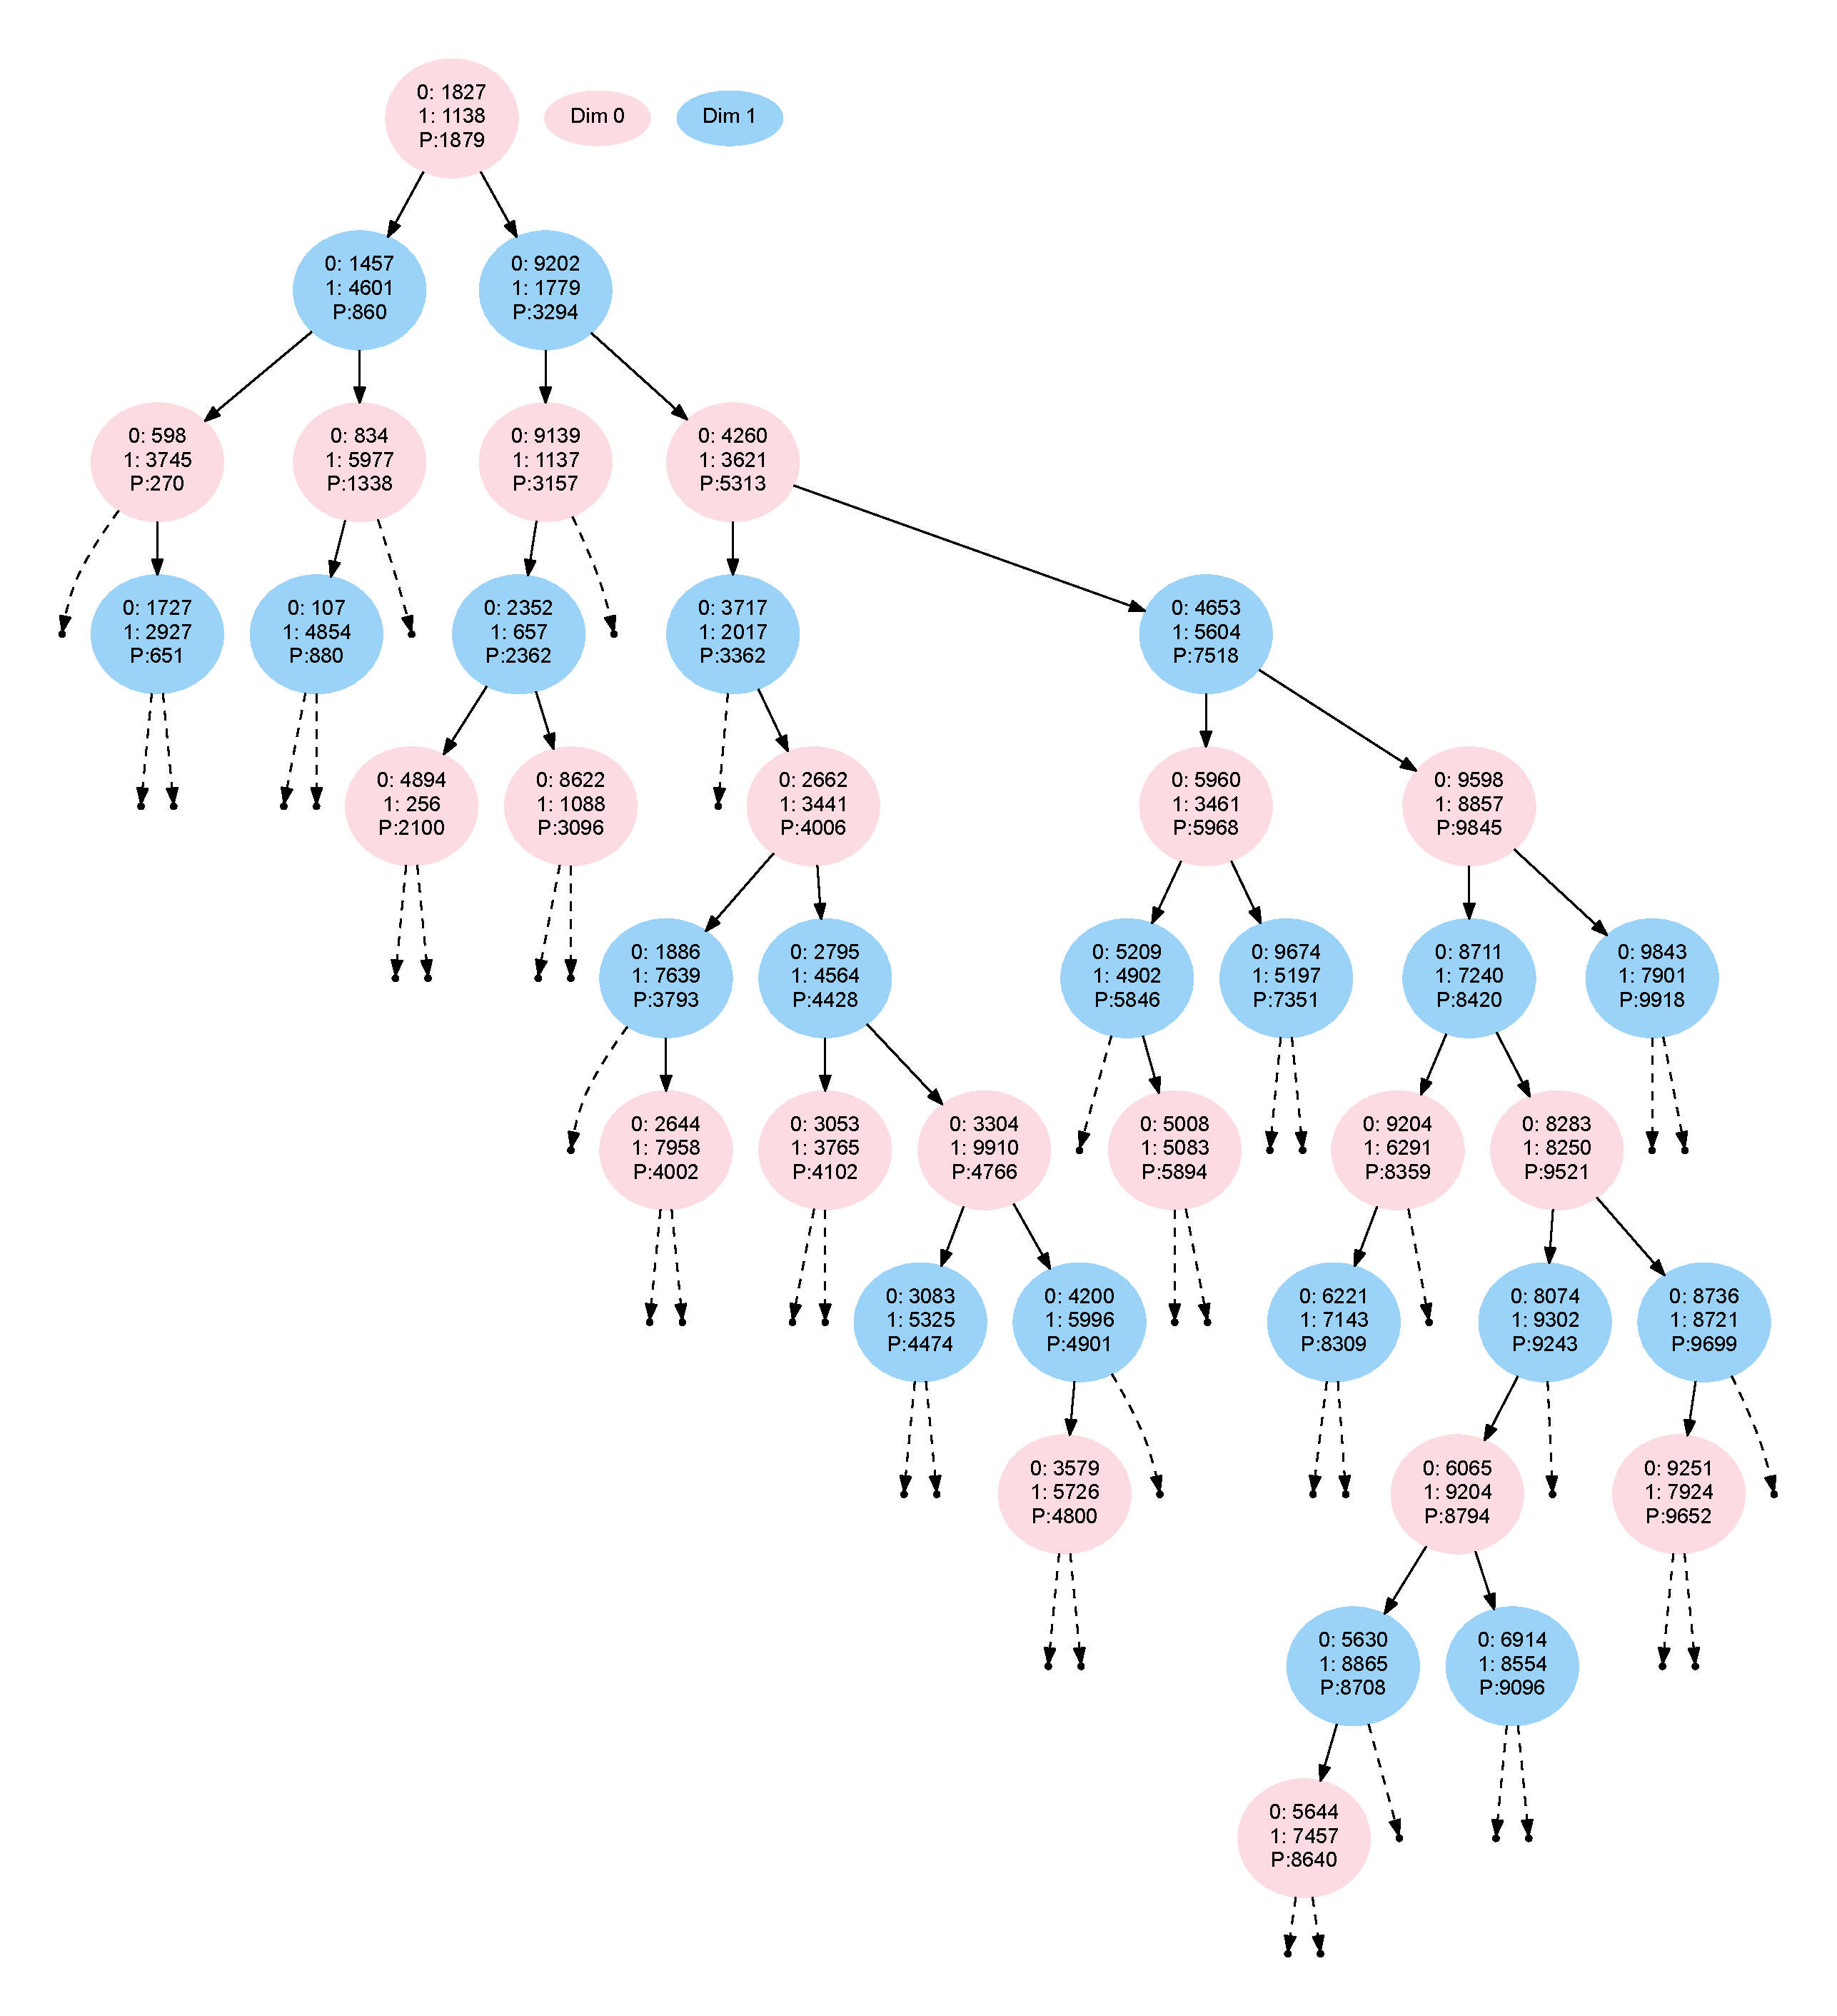
\includegraphics[width=0.2\columnwidth]{Figures/kdtree/kdtree_randomDrandomS}
        }%
	\subfigure[]{%
            \label{fig:randomDsameS}
            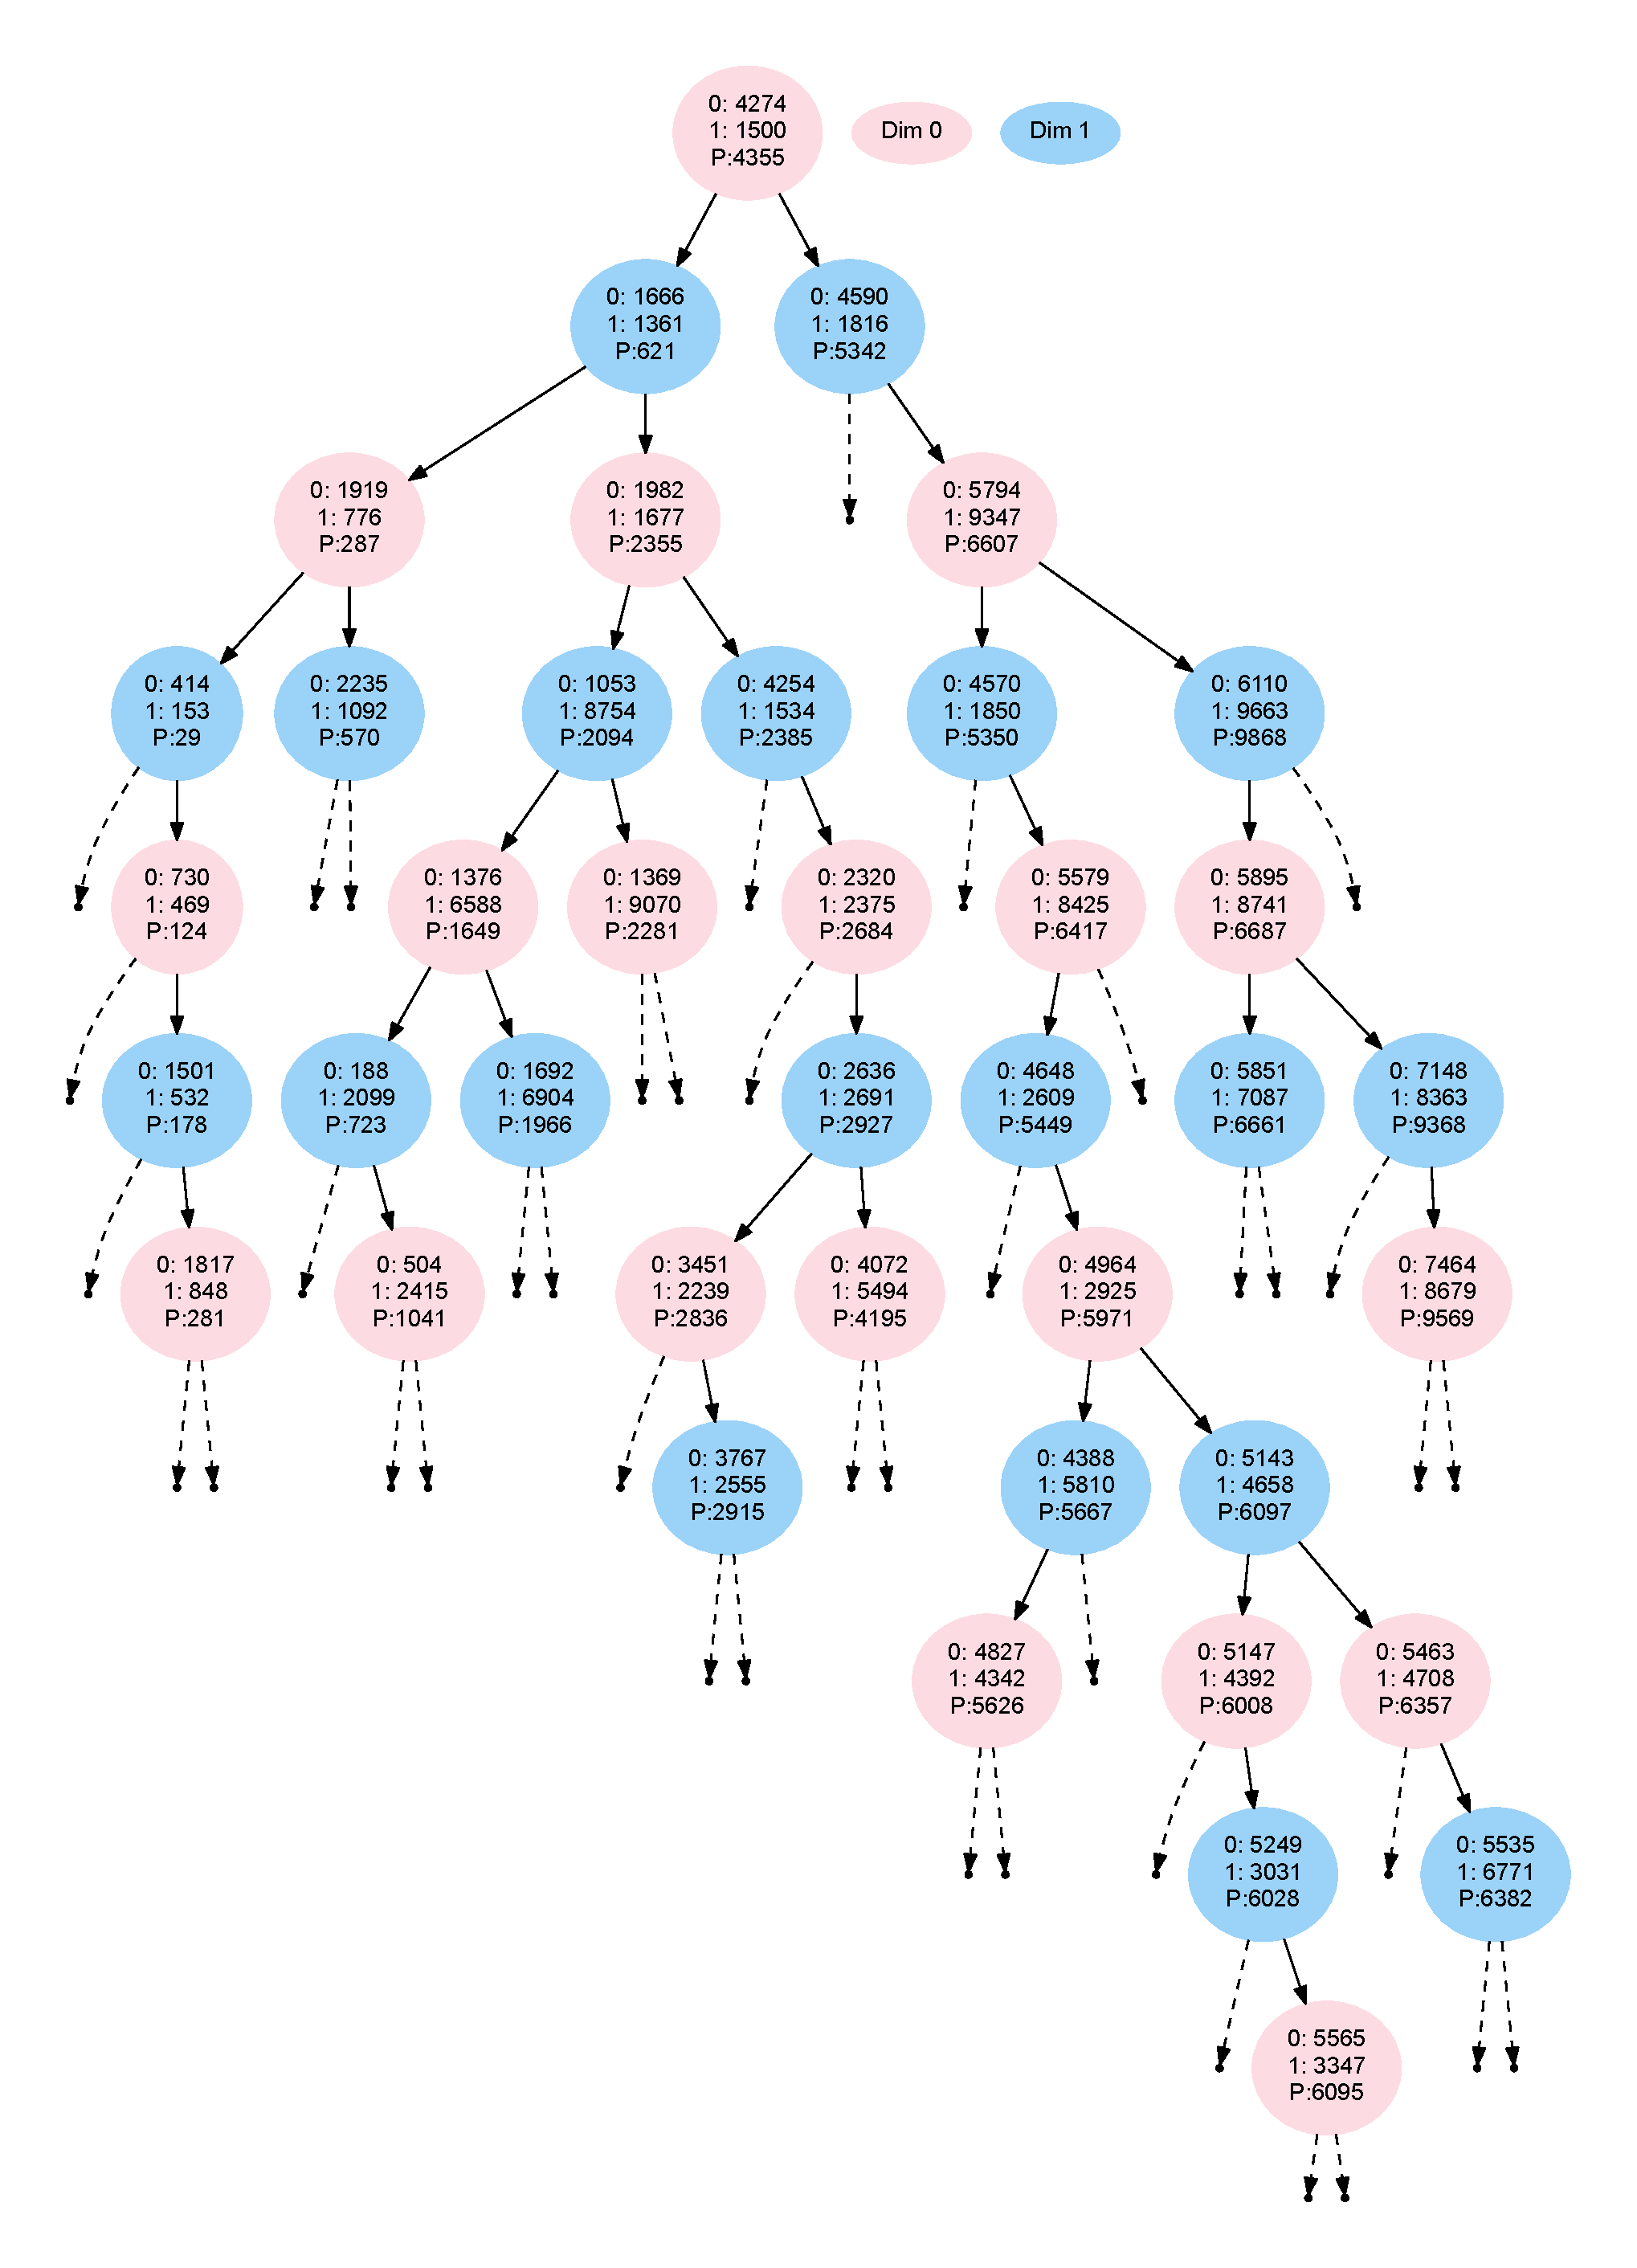
\includegraphics[width=0.2\columnwidth]{Figures/kdtree/kdtree_randomDsameS}
        }%
        \subfigure[]{%
            \label{fig:randomDSBsameS}
            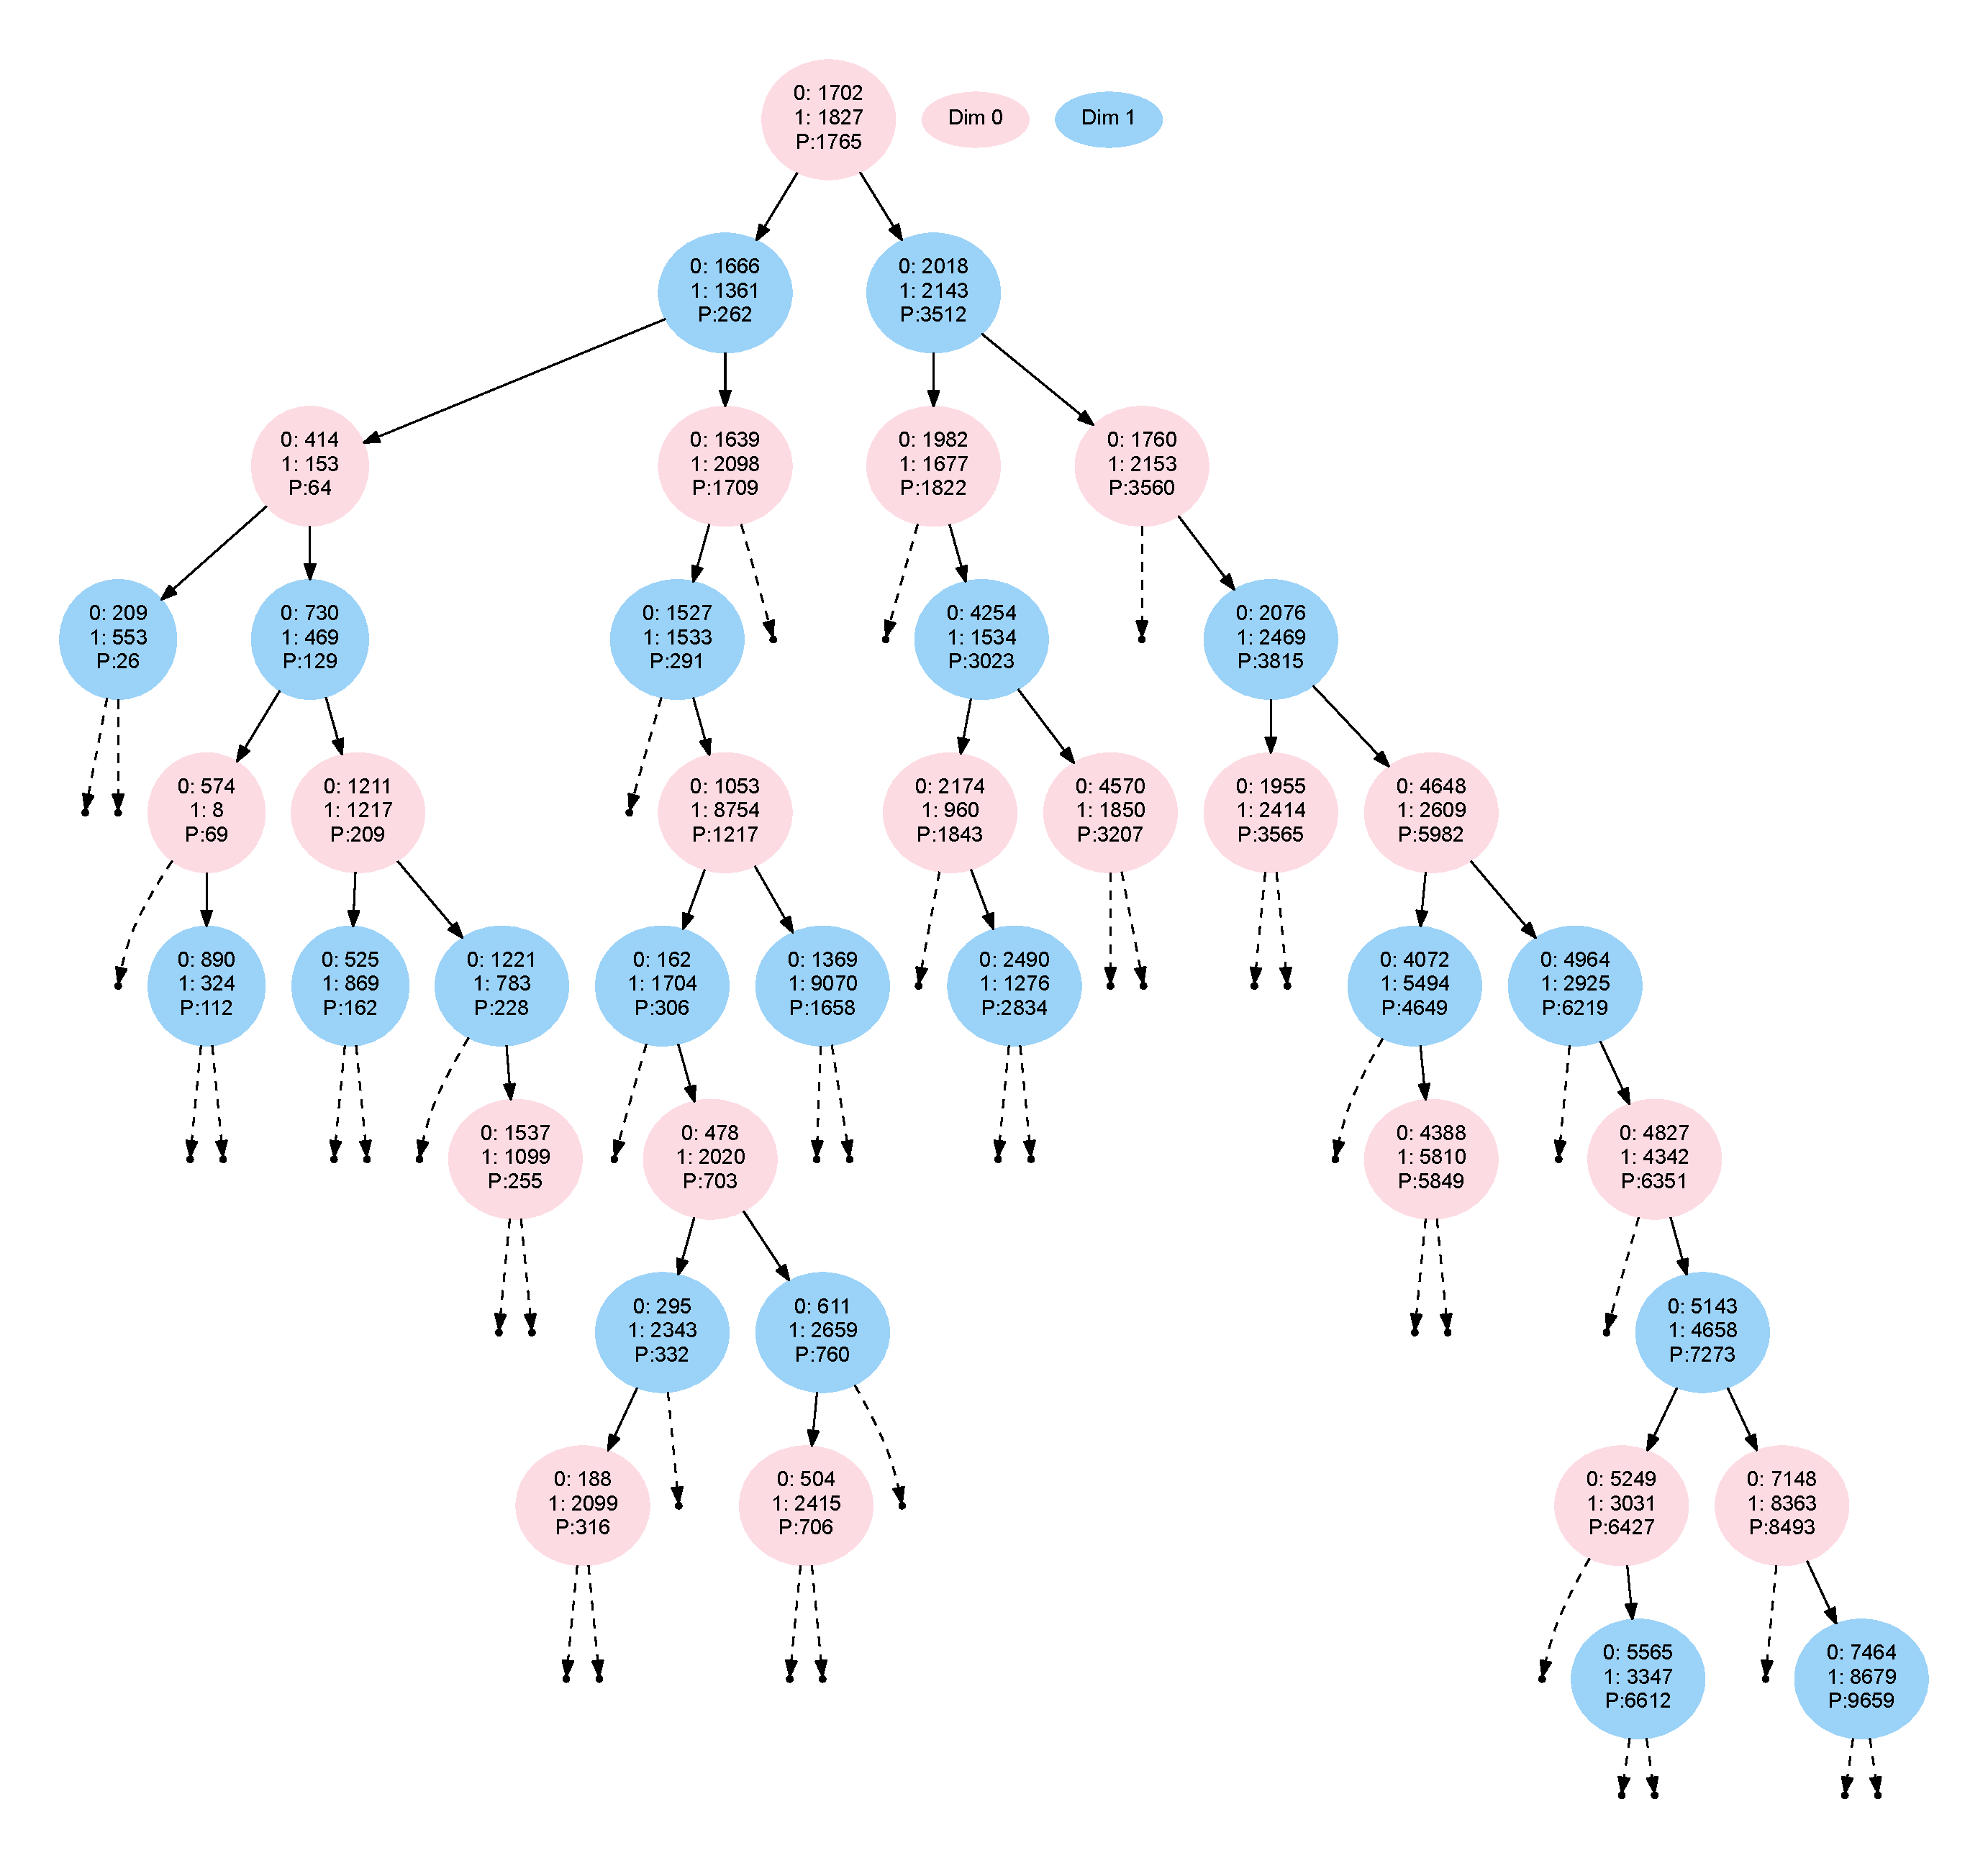
\includegraphics[width=0.2\columnwidth]{Figures/kdtree/kdtree_randomDSBsameS}
        }%
	\subfigure[]{%
            \label{fig:skewedDsameS}
            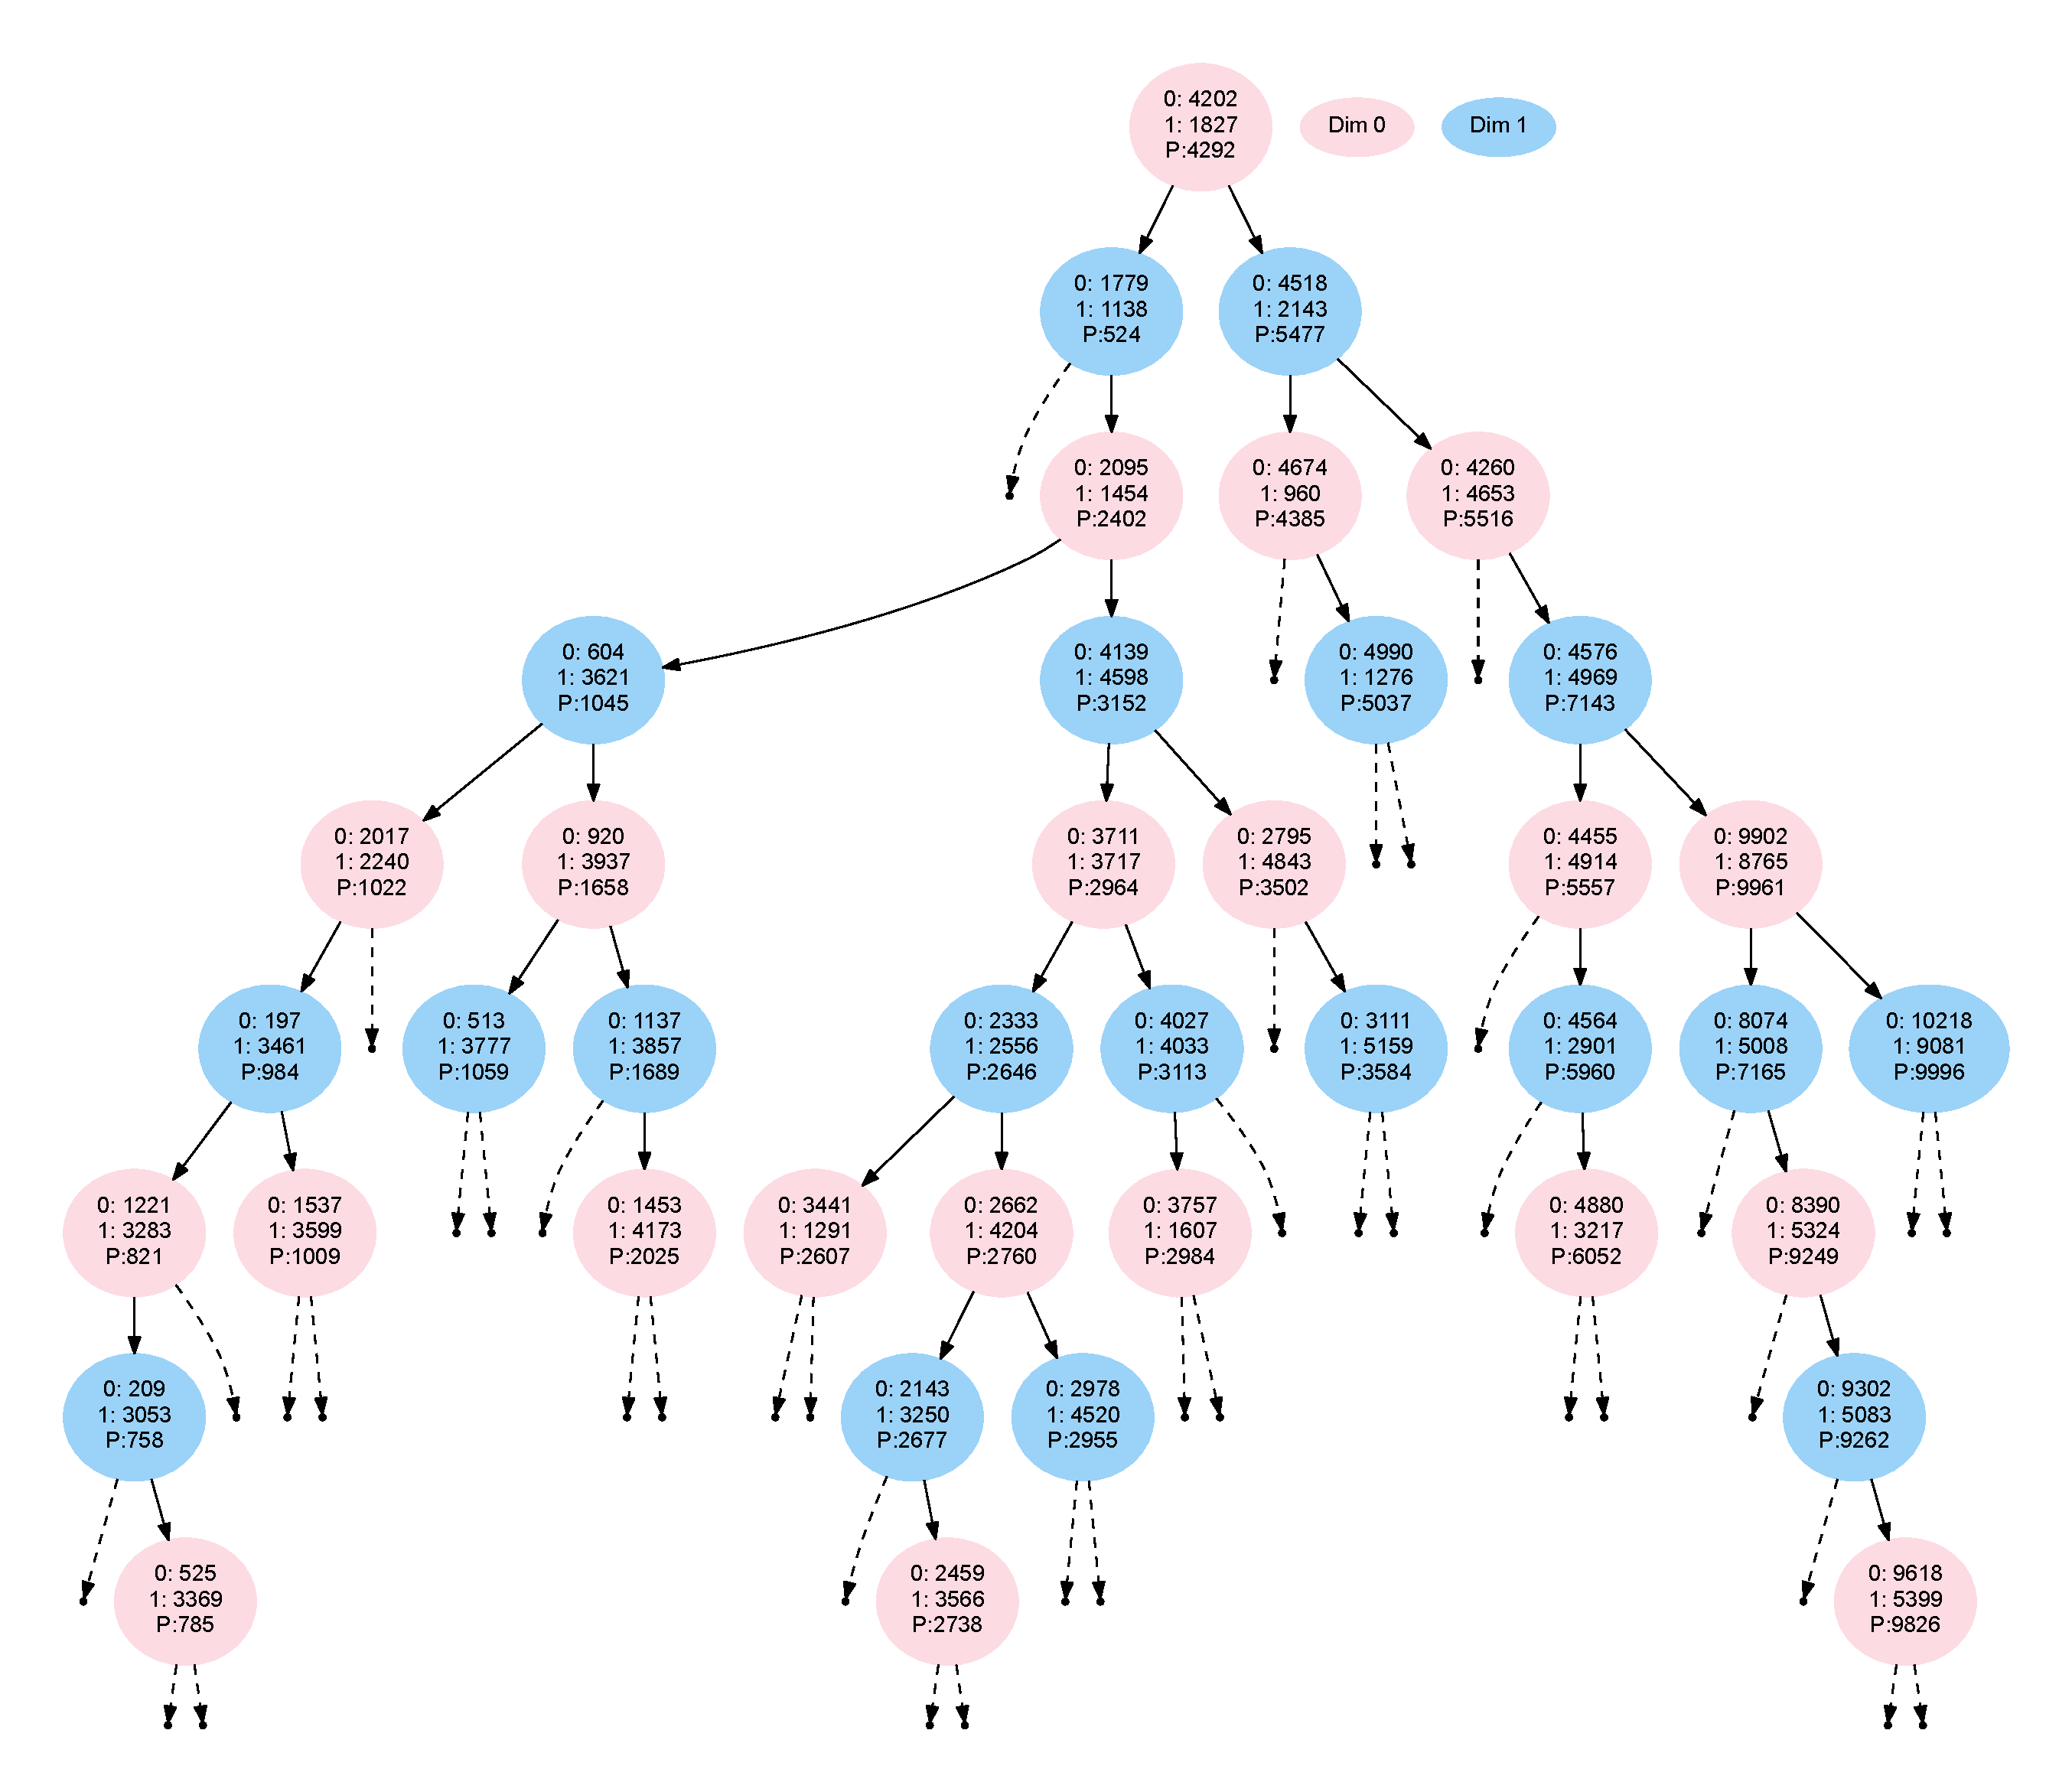
\includegraphics[width=0.2\columnwidth]{Figures/kdtree/kdtree_skewedDsameS}
        }%
        \subfigure[]{%
            \label{fig:sequentialDsameS}
            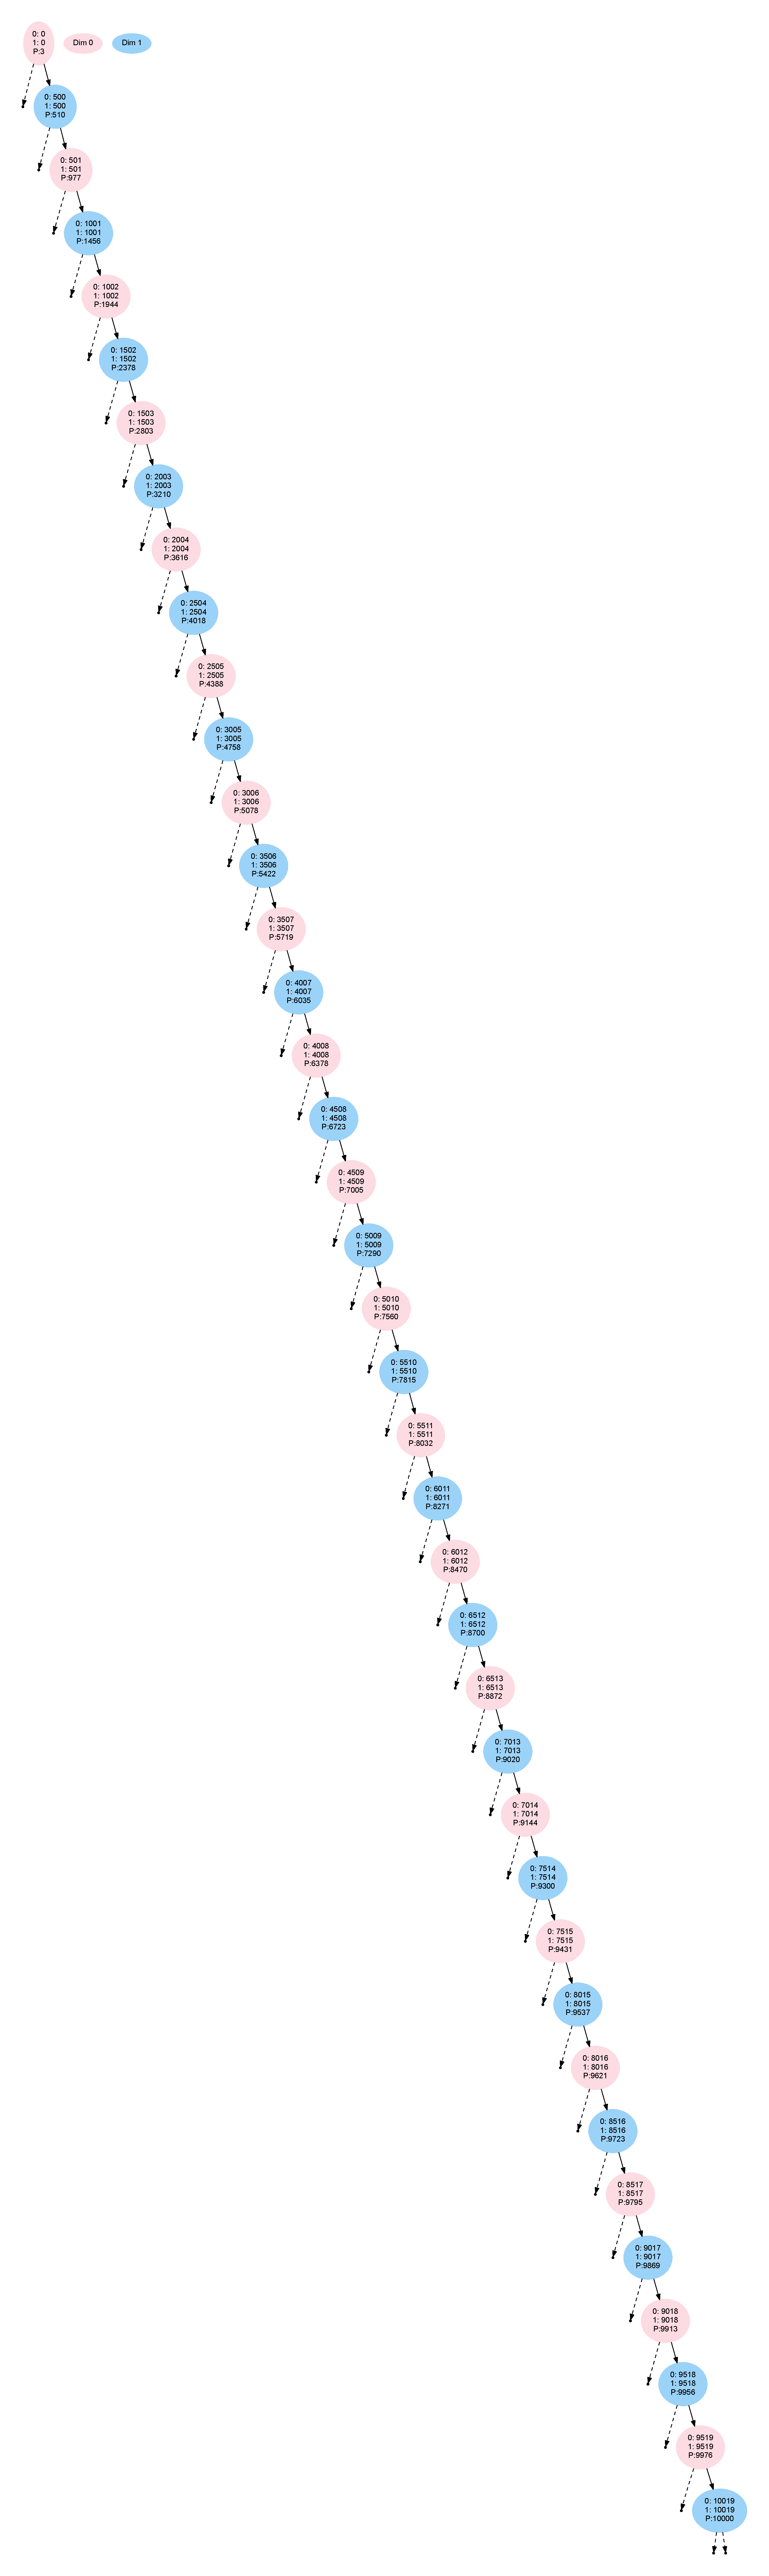
\includegraphics[width=0.2\columnwidth]{Figures/kdtree/kdtree_sequentialDsameS}
        }%
	\subfigure[]{%
            \label{fig:periodicalDsameS}
            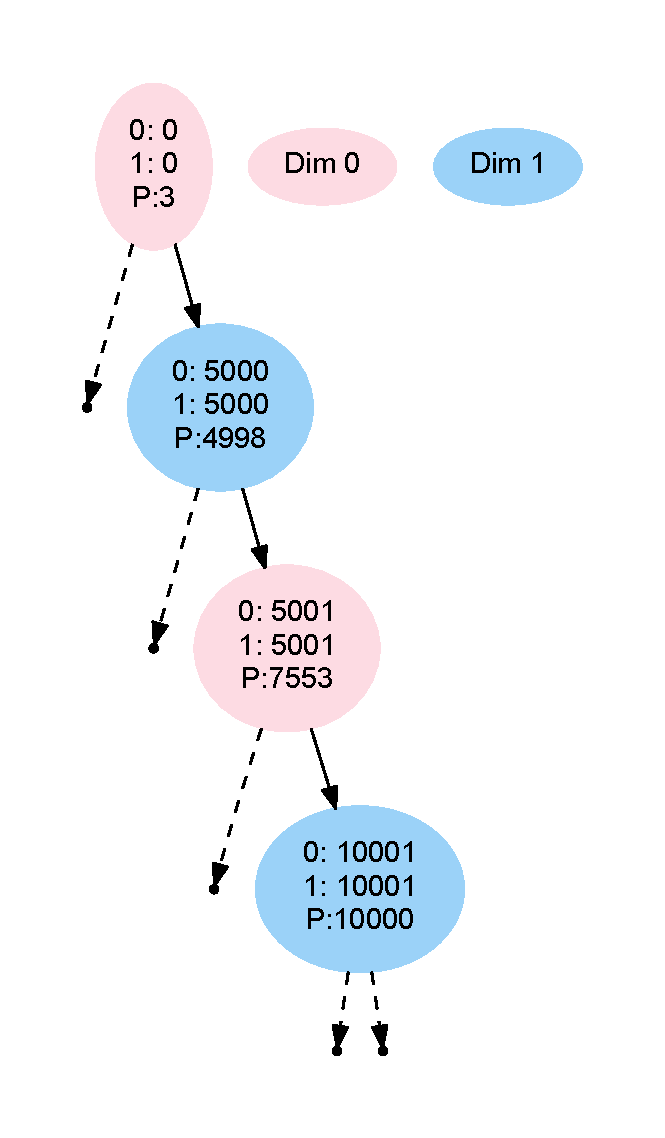
\includegraphics[width=0.2\columnwidth]{Figures/kdtree/kdtree_periodicalDsameS}
        }%
	\subfigure[]{%
            \label{fig:zoominDdifferentS}
            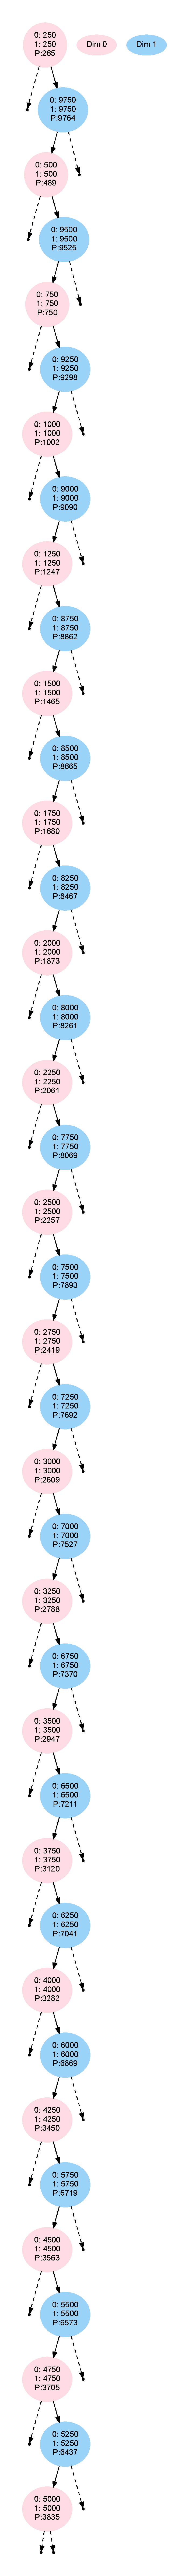
\includegraphics[width=0.2\columnwidth]{Figures/kdtree/kdtree_zoominDdifferentS}
        }
    \caption{kd-tree shape after $20$ queries in different workloads.}
   \label{fig:workload}
    \end{center}
\end{figure*}

